\chapter{Noisy gamma process with unit-to-unit variability} \label{chap:chapter5}

In Chapter~\ref{chap:chapter4}, I discussed how to model a single degradation path using a noisy gamma process postulated through the Bayesian hierarchical modelling framework. I concluded that there is an identifiability issue between the noise and the volatility of the underlying gamma process when there are only a few degradation measurements. A resolution to this preasymptotic nonidentifiability is to add extra information into the analysis of the degradation trace, which can be done by modelling the degradation of a population of $m$ nominaly identical units simultaneously. This raises the question of how the degradation traces of each unit are related to one another. For example, we may assume that all of the units are realisations from the same underlying gamma degradation process.

However, this assumption may be too restrictive in practice since there may be additional variability in their degradation resulting from slight variations in operating conditions or their manufacture. The most common approach to modelling this extra layer of heterogeneity between units beyond what can be explained by the volatility of the gamma degradation process and any covariates is to use a `mixed effects' model, in which some of the parameters of the model---so-called `random effects'---vary between units or individuals, whereas others, the `fixed effects', do not\footnote{This definition is just one of five that \citet{Gelman2005} lists.}. Early examples in the degradation literature include \citet{lu1993} and \citet{lawless2004}, who incorporated random effects into a general path model and gamma process, respectively. A more recent example is \citet{rodriguez-picon2018}, who modelled the GaAs laser dataset that was also analysed by \citet{Meeker1998}. To model the heterogeneity in the degradation paths, \citet{rodriguez-picon2018} incorporate random effects into a noise-free gamma process by specifying the effect in either the mean or variance of the gamma process. By contrast, \citet{peng_2018} follow the methodology of \citet{lawless2004} and specify random effects in the scale parameter of a gamma process.

In this chapter, I show how the hierarchical model for the noisy gamma process can be neatly extended to incorporate unit-to-unit variability through the same BHM formalism and show the advantages of using the mean/coefficient of variation parameterisation in this context. Before going any further, however, it is worth clarifying the terminology that I use. As pointed out above, the terms random and fixed effects are used when mixed effects models are used to describe unit-to-unit variability. However, as \citet{Gelman2005} and \citet{gelman2006} point out, all parameters in a Bayesian analysis are random variables; furthermore, because there is a multiplicity of definitions of fixed and random, such terms can engender considerable confusion [Section~6]\citep{Gelman2005}. Consequently, \citet{Gelman2005} and \citet{gelman2006} make a plea for abandoning these long-used terms in place of more descriptive ones: \emph{varying}, for parameters that differ between groups or units, and \emph{constant}, for parameters that are identical for all groups or units. In this chapter, I simply identify which parameters are common across units, those that are unique to each unit, and, most importantly, the specification of the hierarchical prior distribution(s) for parameters that vary from unit-to-unit.

To demonstrate the models for multiple units, I use a data set from an experiment to measure and then model crack-propagation in the terminal of nominally identical electronic devices originally published by \citet{rodriguez-picon2018}. The non-noisy data are shown in Fig.~\ref{fig:crack-growth-w-noise} as solid lines. To emulate measurement error, I add a small amount of $\mathrm{N}(0, 0.025)$ noise. These new noisy degradation traces are shown as dashed lines in Fig.~\ref{fig:crack-growth-w-noise}. The soft failure of the terminals is considered to be when the crack length reaches 0.4~mm, and we can see from the figure that by the end of the experiment, several units have yet to fail. There are two reasons why such data may be collected \citep{robinson2000}: to estimate the remaining useful life or failure time distributions of units that have yet to fail during operation, or the corresponding quantities for new units. In the analysis that follows, I model the noisy data and show how to estimate such failure time distributions along with uncertainty intervals.

\begin{figure}
   \centering
   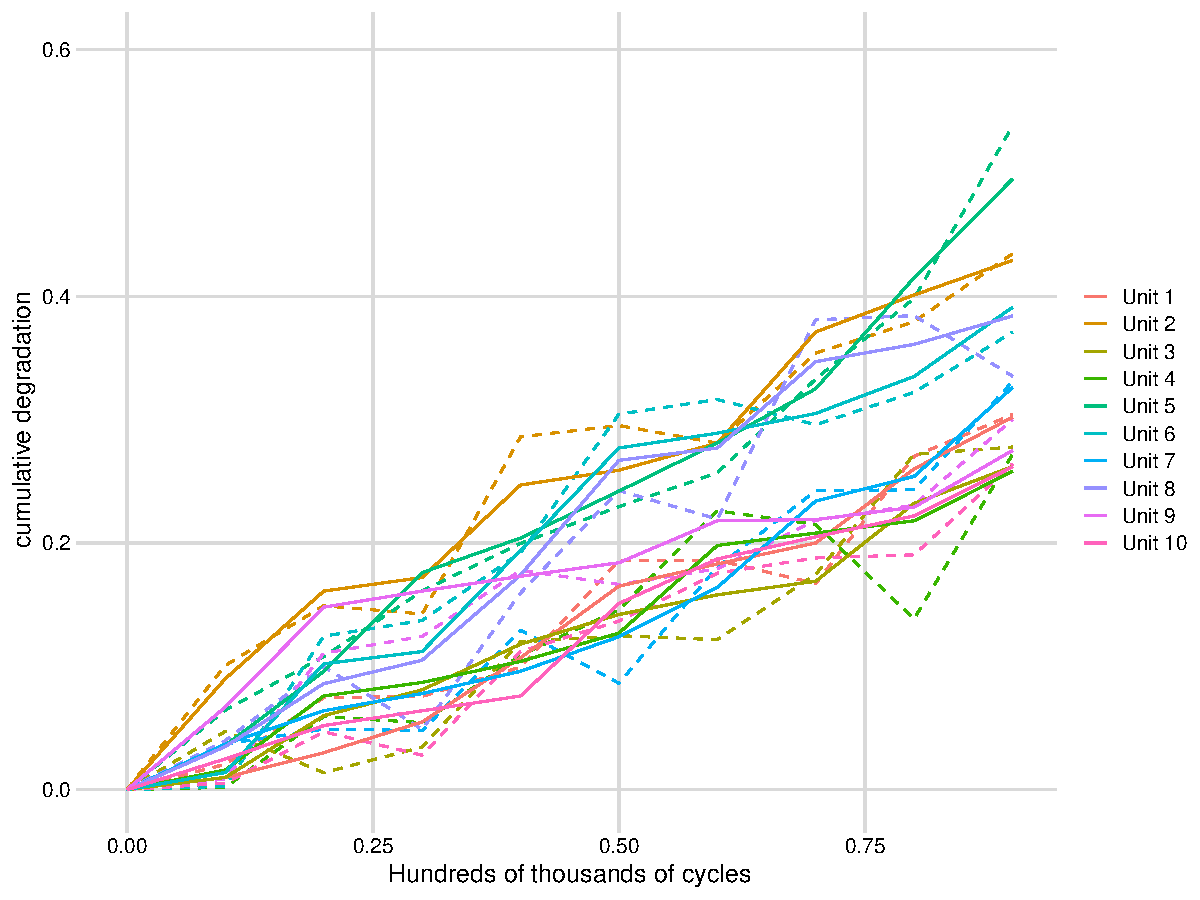
\includegraphics[width=0.95\textwidth]{./figures/ch-5/noisy-crack-growth-data.pdf}
   \caption{Crack-growth propagation data of \citet{rodriguez-picon2018}: original data (solid lines); noisy data (dashed lines).}
   \label{fig:crack-growth-w-noise}
\end{figure}

In the rest of this chapter, I first propose several noisy gamma process models for the multiple noisy degradation traces in Fig.\ref{fig:crack-growth-w-noise} in Sec.~\ref{sec:unit-to-unit-models}; a complete pooling model (i.e., where all parameters are \emph{constant}) and three where either one or both parameters of the gamma process vary across units. In Sec.~\ref{sec:unit-to-unit-sampling}, I then go on to sample from and evaluate the posterior distributions of these models conditioned on the noisy crack-growth data set. The models are also compared using $\mbox{elppd}$ and cross-validation methods. I then show how to construct failure time distributions for a new unit and a unit that is currently under test but yet to fail in Sec.~\ref{sec:unit-to-unit-ft} using both a complete and a partial pooling model. Finally, the findings and conclusions of the analysis are discussed in Sec.~\ref{sec:unit-to-unit-discussion}.

\section{Models for multiple units} \label{sec:unit-to-unit-models}

There are three ways in which we might consider allowing a model for the degradation data in Fig.~\ref{fig:crack-growth-w-noise} to vary, each of which leads to a different form of \emph{pooling}, or, alternatively, of how information is shared or not among the units \citep{Johnson_2022}. The added advantage of the mean/coefficient of variation parameterisation is that it makes it explicit which characteristics of the model we are sharing between units. For example, first, we might make the assumption that for a particular characteristic of the model, such as the mean degradation rate (described by the parameter $\mu$), the units do not contain information that may be relevant to each other and therefore estimate completely separate values of the parameter for each unit; this corresponds to \emph{no pooling}. Secondly, we might assume that all of the units have the same mean wear rate, and the variation that we observe in Fig.~\ref{fig:crack-growth-w-noise} is only due to the volatility of the gamma process and the fact that we have only observed them over such a short period, and hence estimate the parameter $\mu$ by averaging the data from all units---this is \emph{complete pooling}. Finally, although the units are different from each other, they have the same specifications, so we might expect their average degradation rates to share similar characteristics: this supposition can be modelled by allowing the parameter $\mu$ to vary from unit-to-unit yet arise from a common distribution. Doing so results in \emph{partial pooling} of information, which is especially useful when sample sizes are small, but we do not want to make the assumption that all units are identical \cite[Section~13.1]{McElreath_2020}.

Different forms of pooling can be applied to each parameter. For example, \citet{lawless2004} allow the rate parameter of the gamma process to vary from unit-to-unit and assume these unit-specific rate parameters arise from a common distribution whose parameters are estimated from the data (partial pooling) while also assuming that the shape parameter is the same for all units; i.e. completely pooled. The multitude of possible pooling combinations is one reason why it is useful to specify a hierarchical model so that the parameters have separate, clear effects on the outcome---like $\mu$, $\nu$, and $\sigma$ do. By doing so, we can use our understanding of the data-generating process to select a sensible cohort of models to explore.

In the analysis that follows, I confine my exploratory modelling of the crack growth data to models where $\sigma$ is completely pooled, and $\mu$ and $\nu$ are either completely or partially pooled across the units. Since the crack growth data is from a formal experiment, it is reasonable to assume that measurement error in the degradation measurements is constant across the units and observation times and hence to completely pool $\sigma$. Moreover, because the degradation traces are from nominally identical units, it makes sense to assume that their mean wear rate and volatility are in some way related; i.e. either partially or completely pool $\mu$ and $\nu$. Furthermore, if there is no pooling of either $\mu$ or $\nu$, there is no way to make statements about new units without using heuristics and one of the motivations for modelling the crack growth data is to produce reliability estimates for new units. In the next section, I define the complete and partial pooling models that I explore in the rest of the chapter. If it was suspected that the measurement error varied between the units, then the same methods that I describe for varying $\mu$ and $\nu$ in Sec.~\ref{subsec:partial-pooling} bellow could be used for $\sigma$.

\subsection{The complete pooling model}
\label{subsec:complete-pooling}

I denote by $y_{ij}$, $j = 1, 2, \ldots, J$, the measured degradation of $J$ identical units, and without loss of generality, assume that they are measured at the same times $t_i$, $i = 1, 2, \ldots, I$. In a complete pooling model for the crack growth data, both parameters $\mu$ and $\nu$ are completely pooled between the ten units. In other words, each unit is a realisation from the same underlying gamma degradation process. I specify the complete pooling model 
\begin{align*} 
   y_{ij}|z_{ij}, \sigma & \sim \mbox{N}(z_{ij}, \sigma) && \mbox{data model} \\
   \Delta z_{ij}|\mu, \nu & \sim \mbox{Ga} \left( \frac{\Delta t_{i}}{\nu^2}, \frac{1}{\mu \nu^2} \right) && \mbox{process model} \\
   \sigma & \sim \mbox{Unif}(0, 10) && \mbox{parameter model} \\
   \mu & \sim \mbox{N}^{+}(0.5, 0.2) \\
   \nu & \sim t^{+}_3(0, 0.5)
\end{align*}
for the crack growth data. Note that this model is essentially the same model as I explored in Chap.~\ref{chap:chapter4} except there are now multiple realisations from the gamma process for each $\Delta t_{i}$ corresponding to the jump in degradation from each unit. I also use new values of the hyperparameters that are adjusted to the scale of the crack growth phenomenon. These new priors were selected using prior predictive checking.

Figure~\ref{fig:ppc-multi-unit} shows four prior predictive simulations from the noisy crack growth model with complete pooling. In the figure, each simulated dataset contains the same number of units and observations as the true data set in Fig.~\ref{fig:crack-growth-w-noise}. Clearly, the simulations are noticeably different from the true data; in the first simulation, the units wear much faster; in the second and third, the degradation traces are much more volatile; and in the fourth, there is almost no variability between the pathways. However, as I stressed in Sec.~\ref{sec:Bayesian-methods}, the point of performing prior predictive checks is not to tune the prior until it matches the observed data but rather to ensure that the model produces plausible realisations of the data, which appears to be the case here. Interestingly, through the prior predictive simulations, we can see that the volatility of the gamma process with no varying parameters already allows for a reasonable amount of variation in the degradation traces of the units. Next, I explain how I extended the complete pooling model to allow the parameters to vary between units.

\begin{figure}
   \centering
   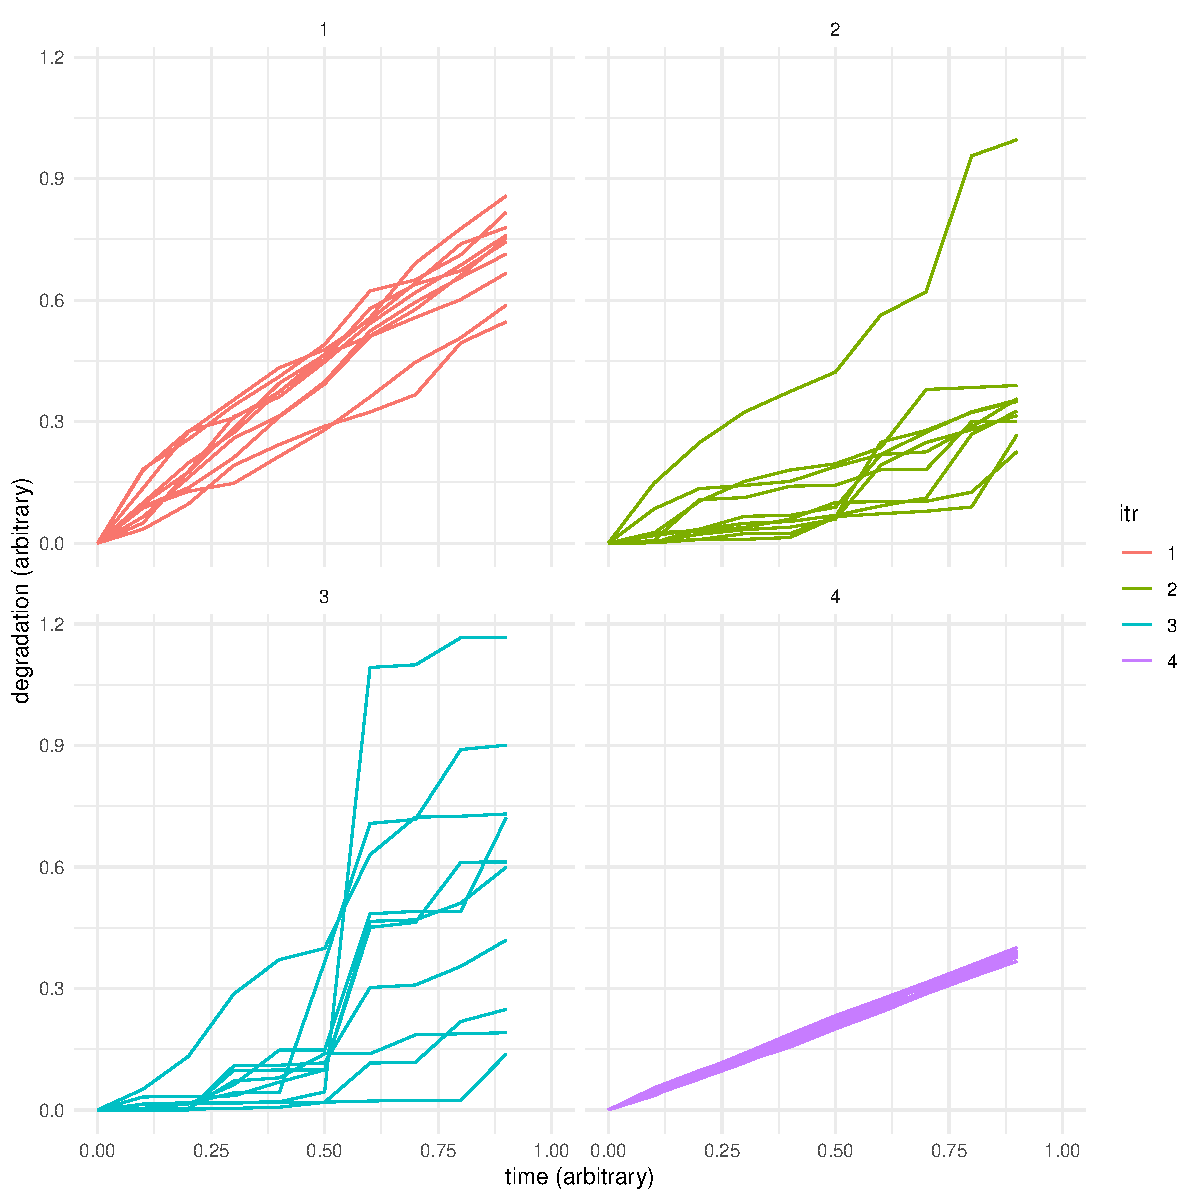
\includegraphics[width=0.95\textwidth]{./figures/ch-5/PPC_multi_unit.pdf}
   \caption{Four non-noisy prior predictive simulations from the complete pooling model. Each simulation contains the same number of units and observations as the crack growth data in Fig.~\ref{fig:crack-growth-w-noise}.}
   \label{fig:ppc-multi-unit} 
\end{figure}

\subsection{Partial pooling models} \label{subsec:partial-pooling}

To incorporate unit-to-unit variability into the complete pooling model above, I assign a hierarchical prior on $\mu$, $\nu$, or both $\mu$ and $\nu$ and then estimate the hyperparameters from the data. I use the general structure
\begin{align*}
   \theta_j| \mu_\theta, \sigma_\theta & \sim \mbox{N}^{+}(\mu_\theta, \sigma_\theta) \\
   \mu_\theta & \sim \prescript{}{\theta}{\pi}\\
   \sigma_\theta & \sim \mbox{Cauchy}^{+}(0, 1) \\
\end{align*}
for the hierarchical prior, where $\theta$ represents the parameter that we are allowing to vary between units, $\theta_j$ are the unit-specific parameters, and $\prescript{}{\theta}{\pi}$ the corresponding prior for that parameter in the complete pooling model. In this hierarchical prior distribution, I assume that the $\theta_j$ arise from a Gaussian distribution whose hyperparameters $\mu_\theta$ and $\sigma_\theta$ are to be estimated. In this way, information is shared across units since a unit-specific estimate of the parameter influences the hyperparameters and, hence, the other unit-specific parameters. I use the same prior for $\mu_\theta$ as the prior used for the completely pooled case of the parameter $\theta$ in the complete pooling model since $\mu_\theta$ now expresses the expected value of the $\theta_j$. Finally, I use a vague truncated Cauchy hyperprior for the standard deviation of the hierarchical prior following the recommendations of \citet[chap.~17]{BDA2020}. These choices are just a general starting point; the more mass close to zero in the hyperprior for $\sigma_\theta$, the more information is pooled between the units \citep{McElreath_2020}, and if I were to use a distribution with heavier tails than a Gaussian, such as the Student's~$t$, then inference about the hyperparameters would be more robust to outlying units \citep[chap.~17]{BDA2020}. Using this general structure of a hierarchical prior, I explore a varying $\mu$ model, varying $\nu$ model and a model where both $\mu$ and $\nu$ vary from unit-to-unit.

\paragraph{Varying $\mu$ model} In the varying $\mu$ model, I am assuming that each of the degradation traces in Fig.\ref{fig:crack-growth-w-noise} arise from different gamma processes where these processes have the same volatility (described by $\nu$) and similar, but not the same, average degradation rates. The varying $\mu$ model is specified as
\begin{align*} 
   y_{ij}|z_{ij}, \sigma & \sim \mbox{N}(z_{ij}, \sigma)  && \mbox{data model} \\
   \Delta z_{ij}|\mu_j, \nu & \sim \mbox{Ga} \left( \frac{\Delta t_{i}}{\nu^2}, \frac{1}{\mu_j \nu^2} \right) && \mbox{process model} \\
   \sigma & \sim \mbox{Unif}(0, 10) && \mbox{parameter model} \\
   \mu_j & \sim \mbox{N}^{+}(\mu_{\mu}, \sigma_{\mu}) \\
   \nu & \sim t^{+}_3(0, 0.5) \\
   \mu_{\mu} & \sim \mbox{N}^{+}(1, 0.2) \\
   \sigma_{\mu} & \sim \mbox{Cauchy}^{+}(0, 1).
\end{align*}

\paragraph{Varying $\nu$ model} In the varying $\nu$ model, I once again assume that each degradation trace is a realisation from a different gamma process. However, this time, I assume that all of these processes share the same average degradation rate $\mu$ but have varying degrees of volatility, $\nu$. I specify the varying $\nu$ model as
\begin{align*} 
   y_{ij}|z_{ij}, \sigma & \sim \mbox{N}(z_{ij}, \sigma)  && \mbox{data model} \\
   \Delta z_{ij}|\mu, \nu_j & \sim \mbox{Ga} \left( \frac{\Delta t_{i}}{\nu_j^2}, \frac{1}{\mu \nu_j^2} \right) && \mbox{process model} \\
   \sigma & \sim \mbox{Unif}(0, 10) && \mbox{parameter model} \\
   \mu & \sim \mbox{N}^{+}(1, 0.2) \\
   \nu_j & \sim \mbox{N}^{+}(\mu_{\nu}, \sigma_{\nu}) \\
   \mu_{\nu} & \sim t^{+}_3(0, 0.5) \\
   \sigma_{\nu} & \sim \mbox{Cauchy}^{+}(0, 1).
\end{align*}

\paragraph{Varying $\mu$ and $\nu$ model} In the final and most flexible model, I assume that the gamma processes that each degradation trace arises from have unique values of $\mu$ and $\nu$. This model where both $\mu$ and $\nu$ are partially pooled is
\begin{align*} 
   y_{ij}|z_{ij}, \sigma & \sim \mbox{N}(z_{ij}, \sigma)  && \mbox{data model} \\
   \Delta z_{ij}|\mu_j, \nu_j & \sim \mbox{Ga} \left( \frac{\Delta t_{i}}{\nu_j^2}, \frac{1}{\mu_j \nu_j^2} \right) && \mbox{process model} \\
   \sigma & \sim \mbox{Unif}(0, 10) && \mbox{parameter model} \\
   \mu_j & \sim \mbox{N}^{+}(\mu_{\mu}, \sigma_{\mu}) \\
   \nu_j & \sim \mbox{N}^{+}(\mu_{\nu}, \sigma_{\nu}) \\
   \mu_{\mu} & \sim t^{+}_3(0, 0.5) \\
   \sigma_{\mu} & \sim \mbox{Cauchy}^{+}(0, 1) \\
   \mu_{\nu} & \sim t^{+}_3(0, 0.5) \\
   \sigma_{\nu} & \sim \mbox{Cauchy}^{+}(0, 1).
\end{align*}

These models can be seen as a set of nested models where the varying $\mu$, varying $\nu$, and complete pooling models are special cases of the model where both $\mu$ and $\nu$ vary. In models where either $\mu$, $\nu$, or both are constant across the different units, the complete pooling is equivalent to a model in which the hyperparameters $\sigma_\mu$ or $\sigma_\nu \longrightarrow 0$ and hence the unit specific parameters are forced to be equal to the mean hyperparameters $\mu_\mu$ or $\mu_\nu$.

\section{Computation, posteriors, and predictive distributions} \label{sec:unit-to-unit-sampling}

I fit all four models with the No-U-Turn sampler. The HMC algorithm is remarkably efficient, particularly for the complete pooling model, and exploring the posterior distributions requires only six chains of length 1000 after a burn-in period of 1000 iterations. The $n_{\mbox{eff}}$ and $\hat{R}$ statistics for the parameters of interest for all four models indicate that, in all cases, the chains have mixed well \citep{Vehtari_2021}, these statistics are shown in Tabs.~\ref{tab:cp}--\ref{tab:pp_both} for the different models. During sampling from the posteriors of the four hierarchical models, some divergent transitions occur---particularly in the models where $\nu$ varies from unit-to-unit. Table~\ref{tab:n_divergent} lists the number of divergent transitions that occur while sampling from the posterior of each model.

In the first part of this section, I summarise the inference from each model and show that all models have been able to reclaim the scale of the measurement error and the true underlying degradation paths from the noisy data. I also investigate the cause of the divergent transitions for the hierarchical models, identifying the cause to be the tight curvature in the posterior distributions where the partial pooling collapses towards the complete pooling case. Posterior predictive checking is used to understand the practical differences between the fitted models. Section~\ref{subsec:modcomp} then compares the four models using the $\hbox{elppd}_{\text{\tiny{LOO-CV}}}$ scoring method described in Chap.~\ref{chap:chapter1} Sec.~\ref{sec:bayesian-background}.

\begin{table}
\centering
\caption{\label{tab:n_divergent}The number of divergent transitions that occure during sampling.}
\centering
\begin{tabular}[t]{lr}
\toprule
model & number of divergent transitions\\
\midrule
\cellcolor{gray!10}{complete pooling} & \cellcolor{gray!10}{0}\\
partial pooling mu & 23\\
\cellcolor{gray!10}{partial pooling nu} & \cellcolor{gray!10}{110}\\
partial pooling mu and nu & 202\\
\bottomrule
\end{tabular}
\end{table}


\paragraph{Complete pooling} The posterior samples from the complete pooling model for parameters $\sigma$, $\mu$, and $\nu$ are summarised in Tab.~\ref{tab:cp}. The model has done a reasonable job at reclaiming the standard deviation of the measurement error (which is $0.025$) since the expected value of $\sigma$ is $0.030$ and the majority of the posterior mass sits between $\sigma = 0.020$ and $\sigma = 0.040$. The BHM also provides posterior distributions of the underlying degradation. These are shown in Fig.~\ref{fig:cp_filtered} as 95\% credible intervals, along with the noisy data and the true underlying degradation traces from which they were generated. As we can see, the credible intervals contain the underlying true degradation over the entire time span for each of the ten units, with few exceptions.

\begin{table}
\centering
\caption{\label{tab:cp}Output from fitting a model with complete pooling to the noisy data of Fig.~\ref{fig:crack-growth-w-noise}. We assume that the data from all units is a manifestation of a single underlying gamma process, and hence the mean and coefficient of variation of the process do not vary from unit-to-unit.}
\centering
\begin{tabular}[t]{lrrrrrr}
\toprule
Parameter & Mean & 2.5\% & 50\% & 97.5\% & $n_{\small{\mbox{eff}}}$ & $\hat{R}$\\
\midrule
\cellcolor{gray!10}{$\sigma$} & \cellcolor{gray!10}{0.03} & \cellcolor{gray!10}{0.02} & \cellcolor{gray!10}{0.03} & \cellcolor{gray!10}{0.04} & \cellcolor{gray!10}{2591} & \cellcolor{gray!10}{1}\\
$\mu$ & 0.38 & 0.33 & 0.38 & 0.44 & 8620 & 1\\
\cellcolor{gray!10}{$\nu$} & \cellcolor{gray!10}{0.21} & \cellcolor{gray!10}{0.15} & \cellcolor{gray!10}{0.21} & \cellcolor{gray!10}{0.28} & \cellcolor{gray!10}{926} & \cellcolor{gray!10}{1}\\
\bottomrule
\end{tabular}
\end{table}


\begin{figure}
   \centering
   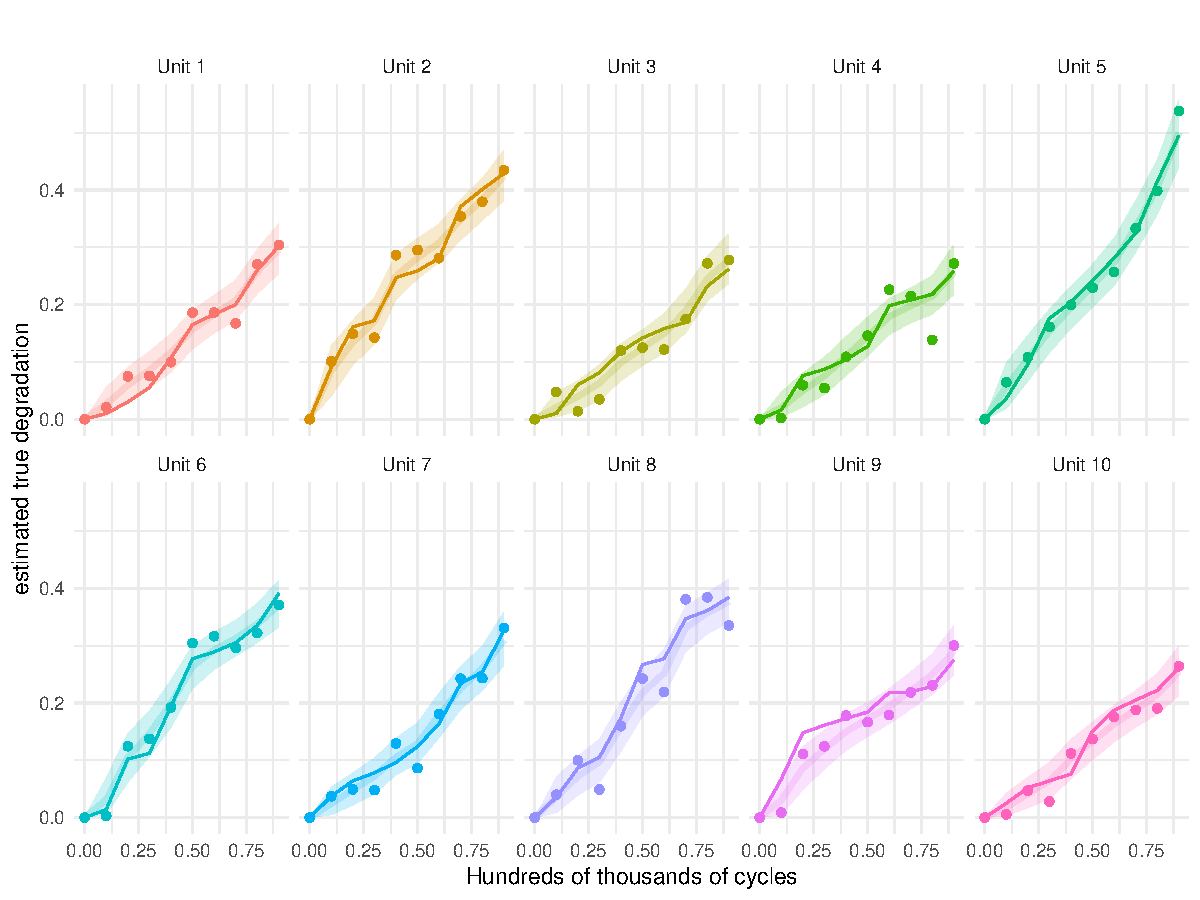
\includegraphics[width=0.8\columnwidth]{./figures/ch-5/plot-cp-filtered.pdf}
   \caption{Marginal posterior distributions of the underlying gamma process from a BHM where all parameters are completely pooled.}
   \label{fig:cp_filtered}
\end{figure}

\paragraph{Varying $\mu$} Table~\ref{tab:pp_mu} shows some summary statistics of the marginal posterior distributions from the varying $\mu$ model for select model parameters, and Fig.~\ref{fig:pp_mu_marg} shows the marginal posterior distributions of the parameters $\sigma$, $\nu$, $\mu_1, \ldots, \mu_{10}$, $\mu_{\mu}$ and $\sigma_{\mu}$. As Tab.~\ref{tab:pp_mu} and Fig.~\ref{fig:pp_mu_marg} show, a posteriori, the mean degradation rates of the units arise from the distribution $\mbox{N}^{+}(0.38, 0.07)$. The small expected standard deviation of $0.07$ indicates that the unit-specific mean degradation rates vary in a relatively narrow range, as the posterior distributions in Fig.~\ref{fig:pp_mu_marg} indicate. In addition, the lower tail of the marginal posterior of $\sigma_\mu$ has a considerable mass near zero, and hence, there is reasonable evidence that the average degradation rate is constant across units. 

Interestingly, the marginal posterior of $\mu_\mu$ is wider relative to $\mu$ in the CP model; however, both have the same mean. The uncertainty intervals of the unit-specific $\mu_j$ are even wider still. A possible reason for this loss of precision is that because I am not making the simplifying assumption that all of the $\mu_j$ are equal, the data do not inform the parameters as strongly since there are now more parameters to estimate in the model, and hence the uncertainty is larger. Additionally, the estimate of $\nu$ has shrunk slightly (particularly in the lower tail). From the shrinkage of $\nu$, it appears that because more of the variability between the traces is being attributed to the variation of the $\mu_j$, the resulting traces are less volatile. Despite these slight changes in inference regarding the mean wear rates and coefficient of variation, the varying $\mu$ model reclaims the true value of $\sigma$ to effectively the same degree as the complete pooling model.

\begin{table}
\centering
\caption{\label{tab:pp_mu}Partial output from fitting a BHM to the noisy data of Fig.~\ref{fig:crack-growth-w-noise} where mean degradation $\mu_j$ varies between units. Only statistics for Units~1--4 are shown.}
\centering
\begin{tabular}[t]{lrrrrrr}
\toprule
Parameter & Mean & 2.5\% & 50\% & 97.5\% & $n_{\small{\mbox{eff}}}$ & $\hat{R}$\\
\midrule
\cellcolor{gray!10}{$\sigma$} & \cellcolor{gray!10}{0.03} & \cellcolor{gray!10}{0.02} & \cellcolor{gray!10}{0.03} & \cellcolor{gray!10}{0.04} & \cellcolor{gray!10}{747} & \cellcolor{gray!10}{1.01}\\
$\mu_1$ & 0.36 & 0.26 & 0.36 & 0.47 & 2150 & 1.00\\
\cellcolor{gray!10}{$\mu_2$} & \cellcolor{gray!10}{0.42} & \cellcolor{gray!10}{0.33} & \cellcolor{gray!10}{0.42} & \cellcolor{gray!10}{0.56} & \cellcolor{gray!10}{954} & \cellcolor{gray!10}{1.00}\\
$\mu_3$ & 0.35 & 0.25 & 0.35 & 0.46 & 1001 & 1.00\\
\cellcolor{gray!10}{$\mu_4$} & \cellcolor{gray!10}{0.34} & \cellcolor{gray!10}{0.23} & \cellcolor{gray!10}{0.34} & \cellcolor{gray!10}{0.45} & \cellcolor{gray!10}{746} & \cellcolor{gray!10}{1.01}\\
\addlinespace
$\nu$ & 0.18 & 0.09 & 0.18 & 0.28 & 248 & 1.03\\
\cellcolor{gray!10}{$\mu_\mu$} & \cellcolor{gray!10}{0.38} & \cellcolor{gray!10}{0.32} & \cellcolor{gray!10}{0.38} & \cellcolor{gray!10}{0.46} & \cellcolor{gray!10}{3079} & \cellcolor{gray!10}{1.00}\\
$\sigma_\mu$ & 0.07 & 0.01 & 0.06 & 0.17 & 343 & 1.01\\
\bottomrule
\end{tabular}
\end{table}


\begin{figure}
   \centering
   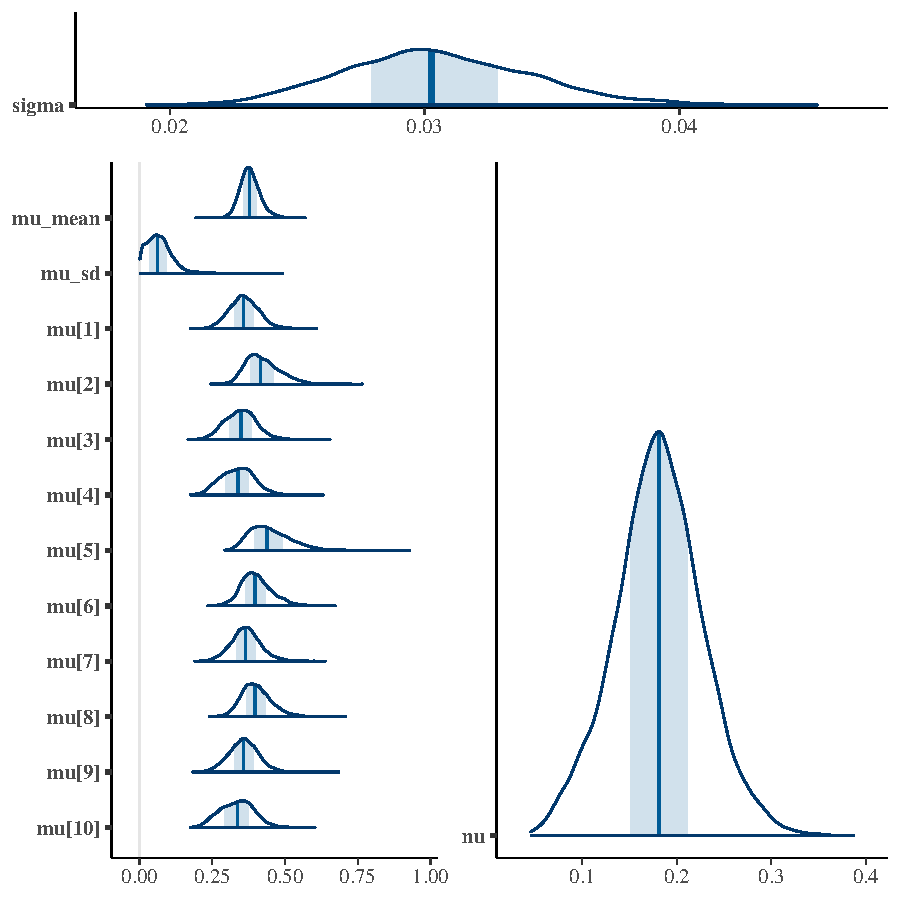
\includegraphics[width=0.95\textwidth]{./figures/ch-5/plot-pp-mu-marg-post-1.pdf}
   \caption{Marginal posterior distributions of parameters from the model where mean degradation rate $\mu_j$ varies from unit-to-unit.}
   \label{fig:pp_mu_marg} 
\end{figure}

During the sampling from the posterior of the varying $\mu$ model, a small number (twenty-three) of divergent transitions occur. Figure~\ref{fig:pp_mu_pairs} show the pairs plots of the samples from the posterior for the parameters $\mu_1$, $\mu_2$, $\mu_\mu$, and $\sigma_\mu$. The twenty-three divergent transitions are plotted in red in the bivariate scatter plots. In the plots (particularly those in the lower off-diagonal), the divergent trajectories tend to occur for very small values of $\sigma_\mu$. This pattern suggests that in the area of the posterior where the partial pooling model collapses towards the simpler complete pooling case---when $\mu_\mu = \mu_1 = \ldots = \mu_{10}$ and $\sigma_\mu = 0$---there is tight curvature, and hence the sampler starts to misbehave. To confirm this hypothesis, Fig.~\ref{fig:pp_mu_parcoord} show the parallel coordinate plot for $\sigma$, $\mu_\mu$, $\mu_1$, \ldots, $\mu_{10}$, and $\sigma_\mu$ with the non-divergent traces plotted in blue and the divergent traces plotted in red. Tracking the divergent traces through the parameter space, it is clear that the divergencies occur when all the unit specific $\mu_j$ are very close to the mean hyperparameter $\mu_\mu$ and the standard deviation hyperparameter is very close to zero.

\begin{figure}
   \centering
   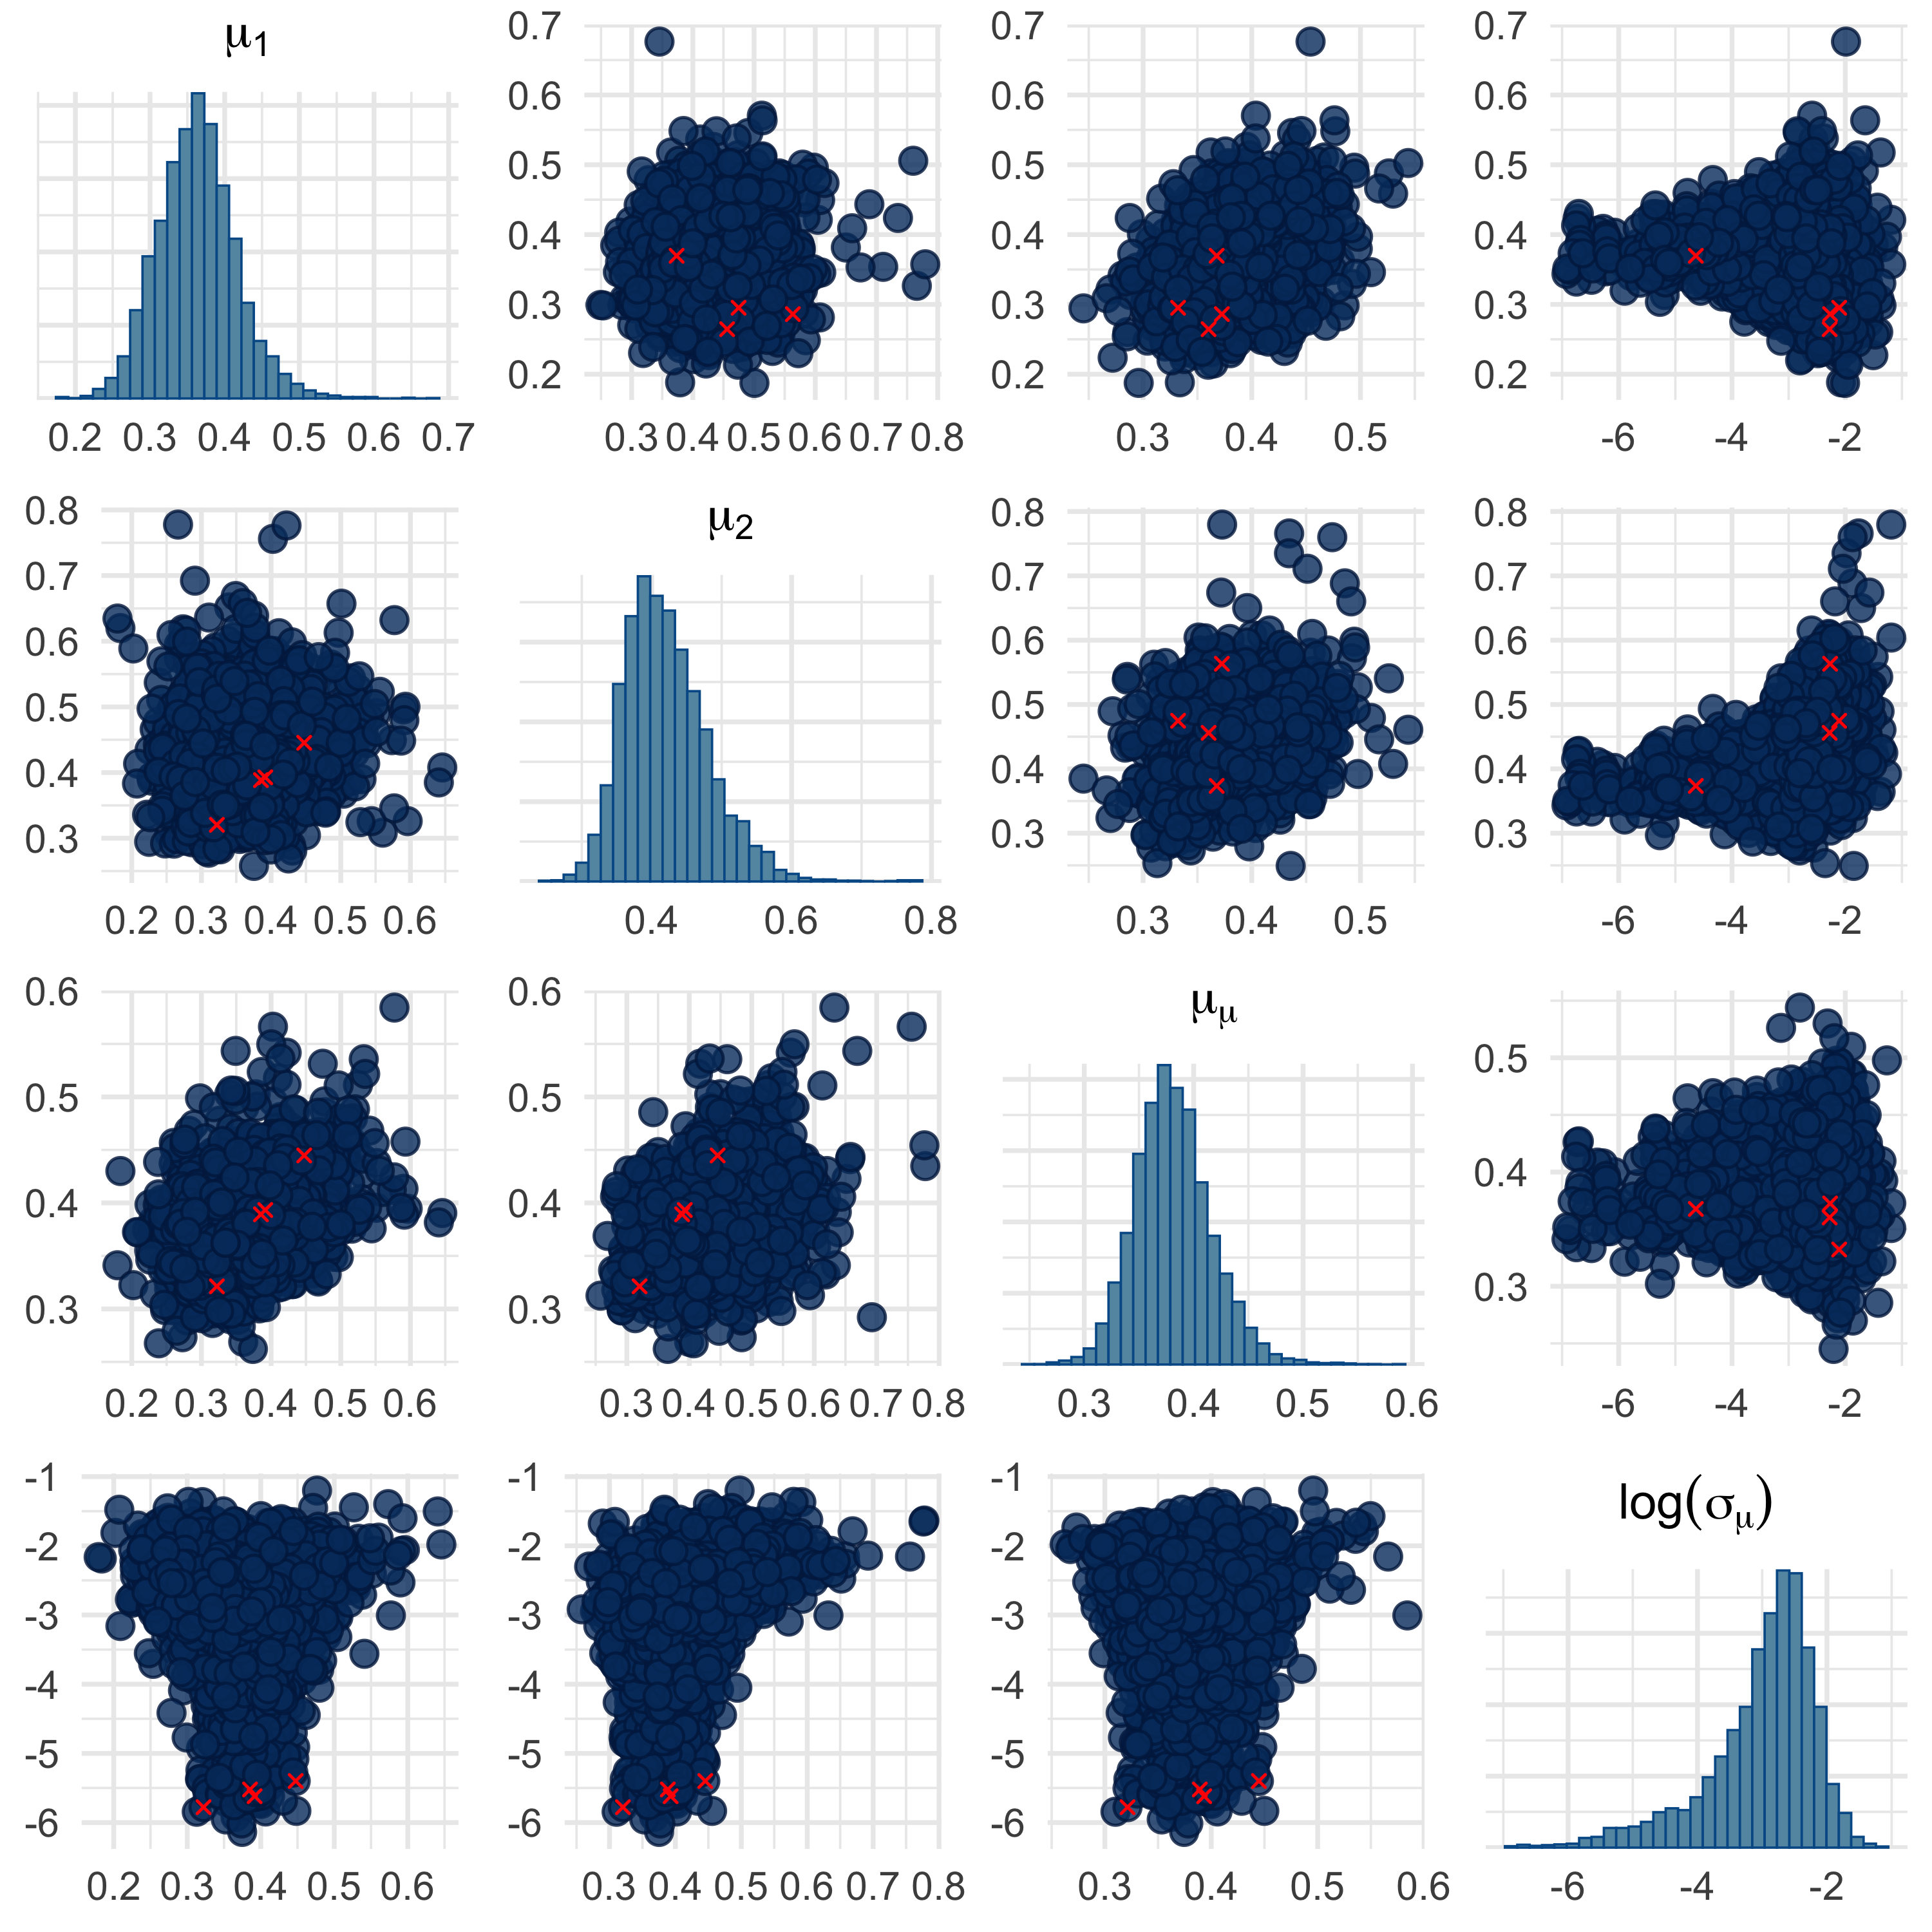
\includegraphics[width=0.95\textwidth]{./figures/ch-5/plot-pp-mu-pairs.png}
   \caption{A pairs plot of the posterior samples of $\mu_1$, $\mu_2$, $\mu_\mu$, and $\log(\sigma_\mu)$ from the varying $\mu$ model. In each bivariate plot, divergencies are plotted in red.}
   \label{fig:pp_mu_pairs} 
\end{figure}

\begin{figure}
   \centering
   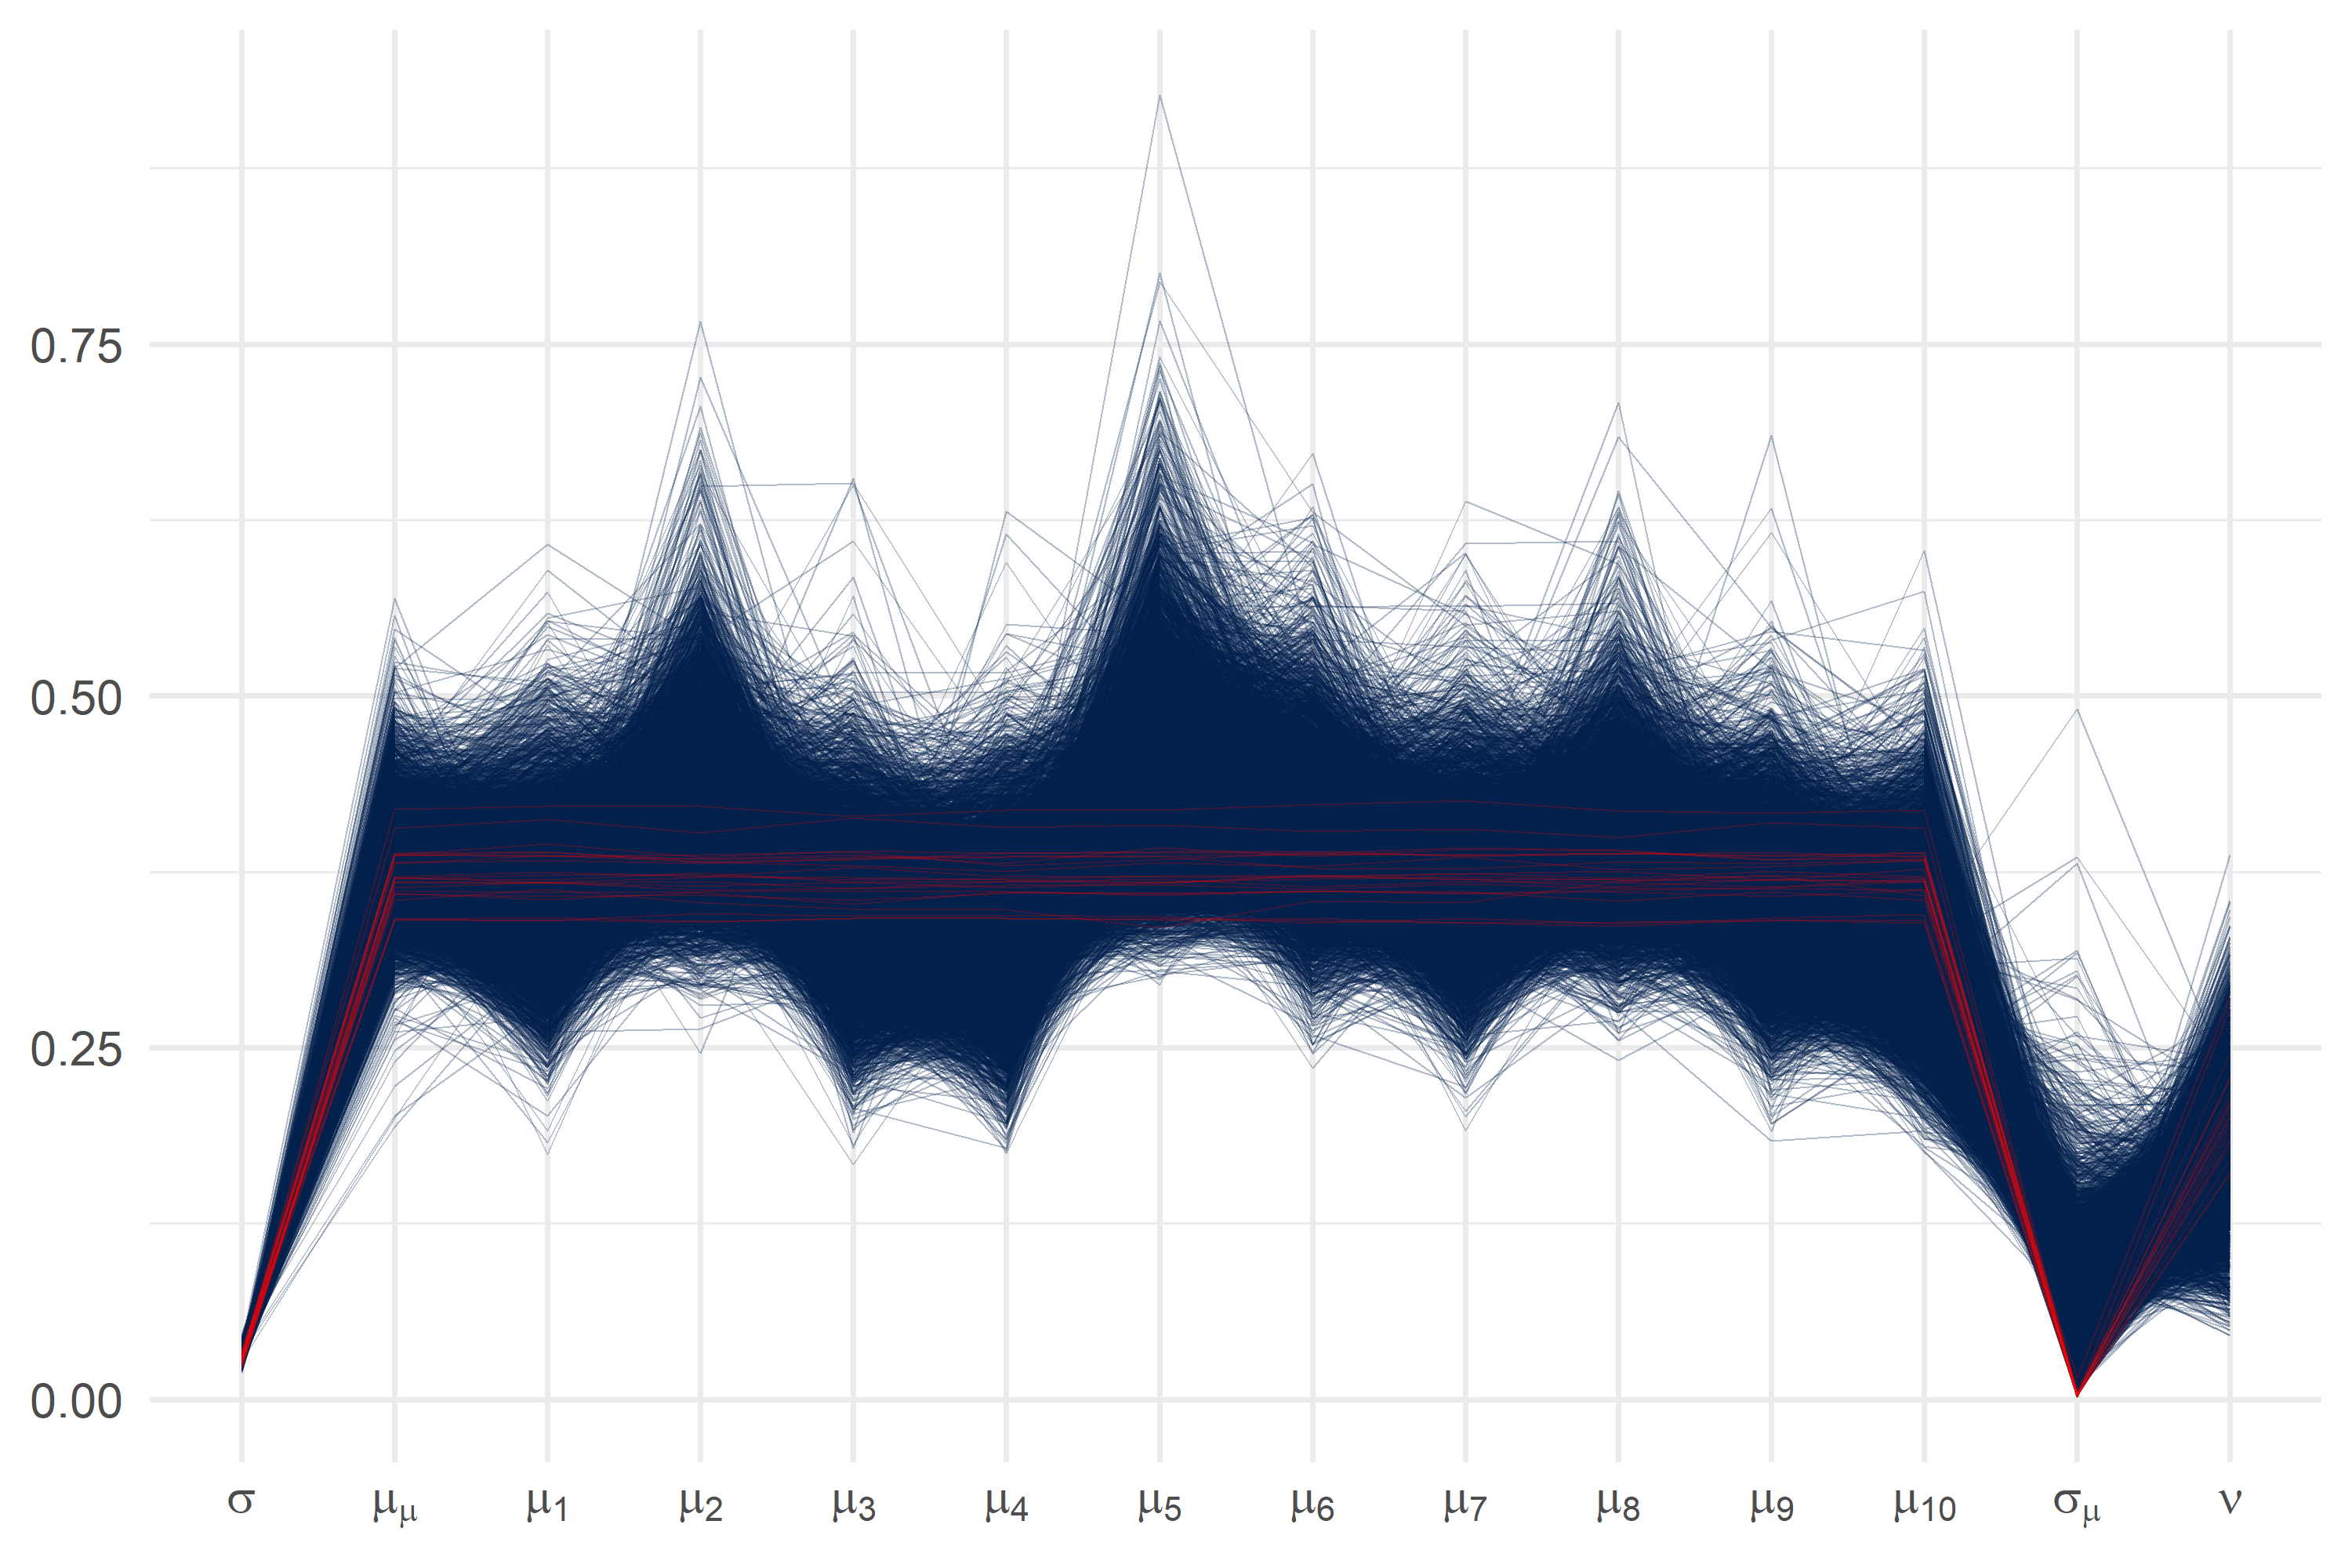
\includegraphics[width=0.95\textwidth]{./figures/ch-5/plot-pp-mu-parcoord.png}
   \caption{Parallel coordinate plot for the parameters and hyper parameters of the varying $\mu$ model. The divergent traces are plotted in red.}
   \label{fig:pp_mu_parcoord} 
\end{figure}

Despite the issues with sampling, the varying $\mu$ model's posterior predictive distributions for the reclaimed `non-noisy' degradation traces match the true degradation traces of the units very closely. Figure~\ref{fig:pp_mu_filtered} shows the posterior predictive distributions of each unit's degradation from the varying $\mu$ model. Like with the complete pooling case, the varying $\mu$ model's the 95\% posterior predictive intervals for the underlying degradation contain the true non-noisy degradation traces most of the time.

\begin{figure}
   \centering
   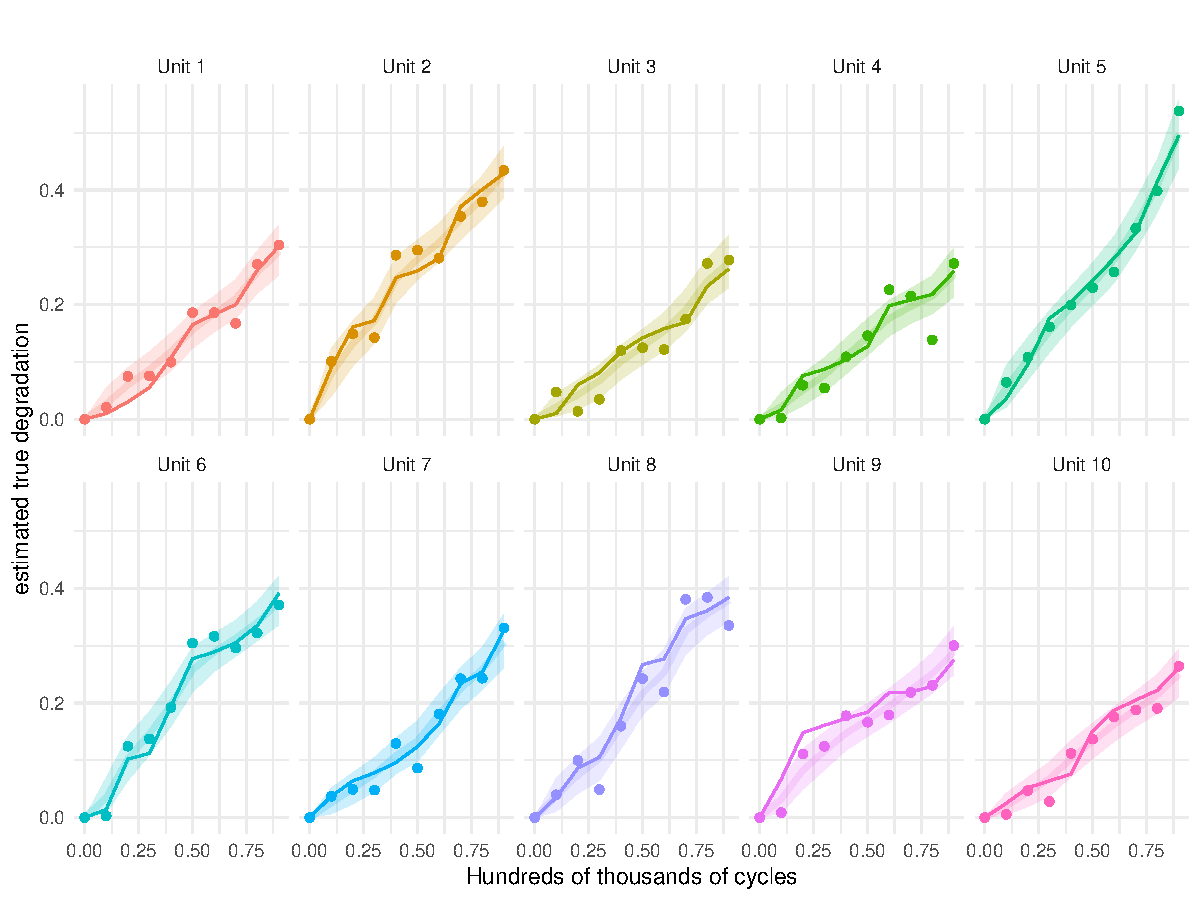
\includegraphics[width=0.8\columnwidth]{./figures/ch-5/plot-pp-mu-filtered.pdf}
   \caption{Marginal posterior distributions of the underlying gamma process from a BHM where mean degradation rate $\mu_j$ varies from unit-to-unit.}
   \label{fig:pp_mu_filtered}
\end{figure}

\paragraph{Varying $\nu$} When $\nu$ is allowed to vary between units instead of $\mu$, all of the $\nu_j$ are effectively equal to the mean $\mu_\nu$, resulting in most of the mass of $\sigma_\nu$ being very close to zero; Tab.~\ref{tab:pp_nu}. In other words, there is little evidence that $\nu$ varies unit-to-unit. Like in the posterior of the varying $\mu$ model, the expected value of the hierarchical prior, in this case, $\mu_\nu$, is effectively the same as the expected value of the parameter in the complete pooling posterior, $\nu$, and the uncertainty intervals are slightly wider in the partial pooling case. As for the completely pooled parameters, the marginal posteriors of $\mu$ in Tab.~\ref{tab:pp_nu} and~\ref{tab:cp} are almost identical, as are the marginal posteriors of $\sigma$. The posterior predictive distributions of the degradation traces (not shown) also look similar to the complete pooling and varying $\mu$ cases.

\begin{table}
\centering
\caption{\label{tab:pp_nu}Partial output from fitting a BHM to the noisy data of Fig.~\ref{fig:crack-growth-w-noise} where the coefficient of variation $\nu_j$ varies between units. Only statistics for Units~1--4 are shown.}
\centering
\begin{tabular}[t]{lrrrrrr}
\toprule
Parameter & Mean & 2.5\% & 50\% & 97.5\% & $n_{\small{\mbox{eff}}}$ & $\hat{R}$\\
\midrule
\cellcolor{gray!10}{$\sigma$} & \cellcolor{gray!10}{0.03} & \cellcolor{gray!10}{0.02} & \cellcolor{gray!10}{0.03} & \cellcolor{gray!10}{0.04} & \cellcolor{gray!10}{1959} & \cellcolor{gray!10}{1.00}\\
$\nu_1$ & 0.21 & 0.11 & 0.21 & 0.32 & 713 & 1.00\\
\cellcolor{gray!10}{$\nu_2$} & \cellcolor{gray!10}{0.23} & \cellcolor{gray!10}{0.14} & \cellcolor{gray!10}{0.22} & \cellcolor{gray!10}{0.34} & \cellcolor{gray!10}{784} & \cellcolor{gray!10}{1.01}\\
$\nu_3$ & 0.23 & 0.14 & 0.22 & 0.35 & 691 & 1.01\\
\cellcolor{gray!10}{$\nu_4$} & \cellcolor{gray!10}{0.23} & \cellcolor{gray!10}{0.13} & \cellcolor{gray!10}{0.22} & \cellcolor{gray!10}{0.35} & \cellcolor{gray!10}{729} & \cellcolor{gray!10}{1.01}\\
\addlinespace
$\mu$ & 0.38 & 0.32 & 0.38 & 0.44 & 2645 & 1.00\\
\cellcolor{gray!10}{$\mu_\nu$} & \cellcolor{gray!10}{0.22} & \cellcolor{gray!10}{0.15} & \cellcolor{gray!10}{0.22} & \cellcolor{gray!10}{0.31} & \cellcolor{gray!10}{506} & \cellcolor{gray!10}{1.01}\\
$\sigma_\nu$ & 0.04 & 0.00 & 0.03 & 0.11 & 344 & 1.02\\
\bottomrule
\end{tabular}
\end{table}


Like the varying $\mu$ model, divergent transitions occur while sampling from the posterior of the varying $\nu$ model. However, there are almost five times more divergencies when fitting the varying $\nu$ model: Tab.~\ref{tab:n_divergent}. Figure~\ref{fig:pp_nu_parcoord} shows the parallel coordinate plot of the MCMC draws for the parameters $\sigma$, $\mu_\nu$, $\nu_1$, \ldots, $\nu_{10}$, and $\sigma_\nu$. Like with varying $\mu$ model, the divergent transitions diagnose a degenerate area in the posterior around $\mu_\nu = \nu_1 = \ldots = \nu_{10}$ and $\sigma_\nu = 0$. In the case of the varying $\nu$ model, there is even more posterior mass around this area since there is little evidence that $\nu$ should vary from unit to unit, and so a higher number of divergent transitions occur.

\begin{figure}
   \centering
   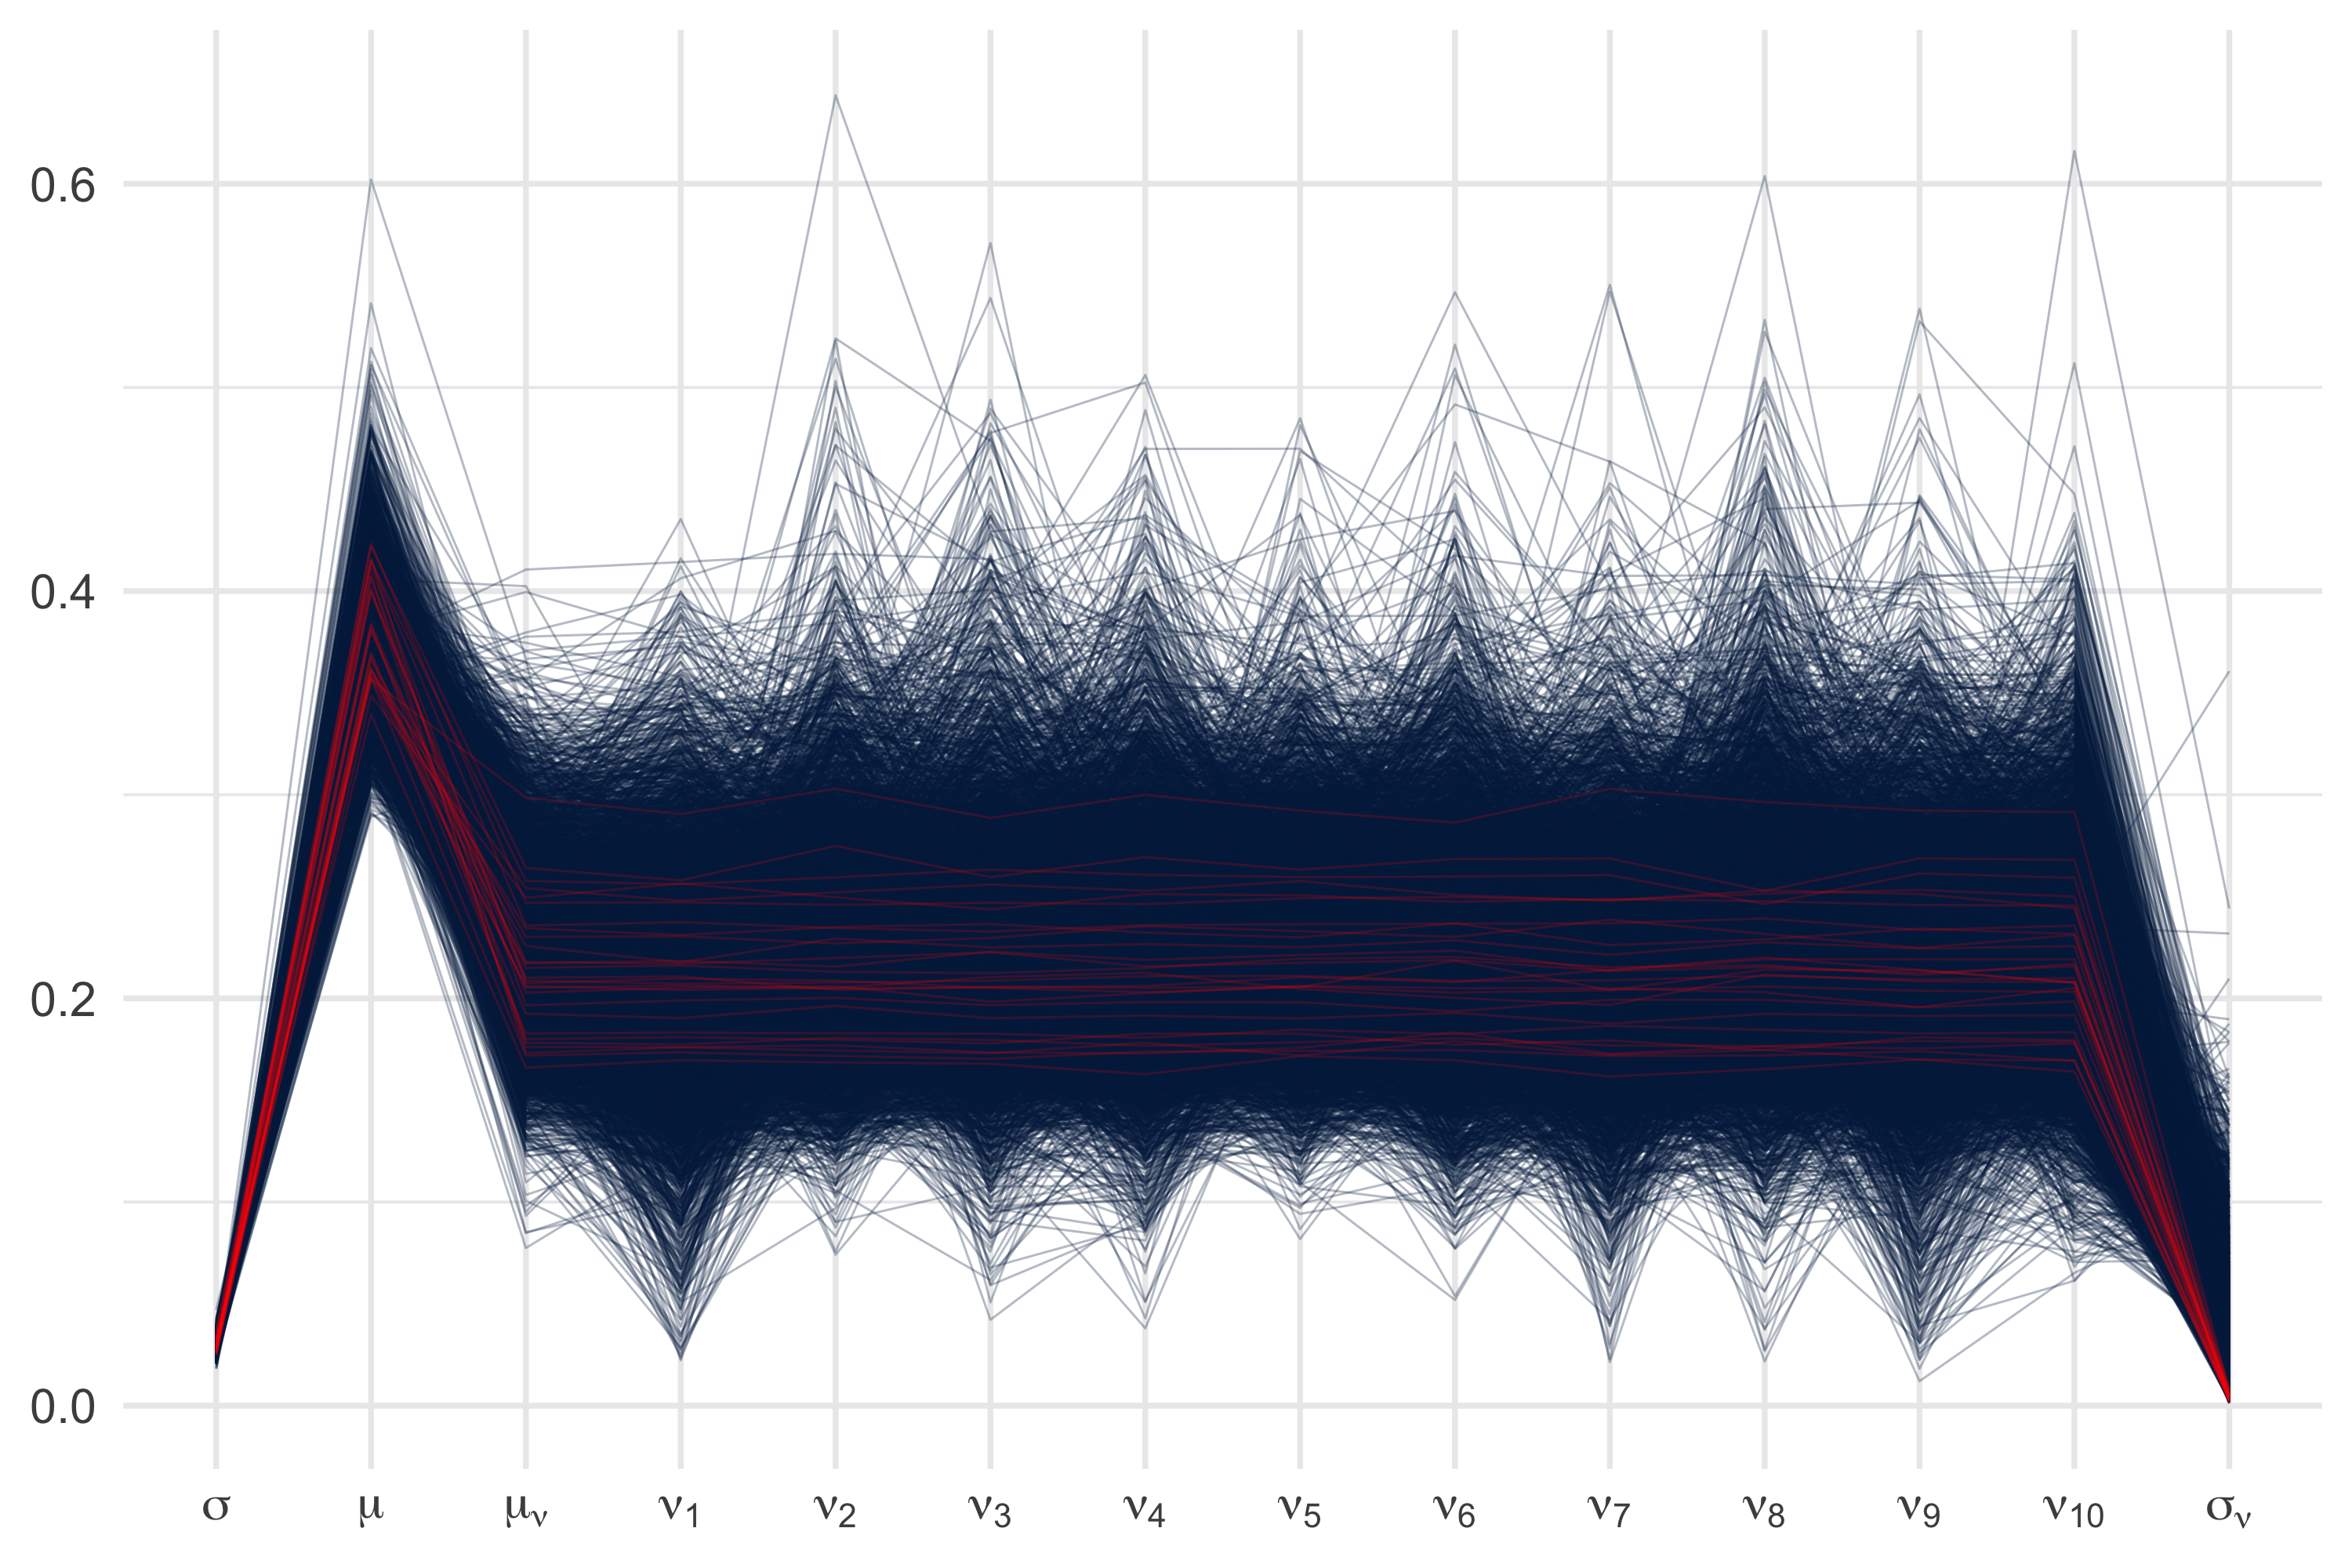
\includegraphics[width=0.95\textwidth]{./figures/ch-5/plot-pp-nu-parcoord.png}
   \caption{Parallel coordinate plot for the parameters and hyper parameters of the varying $\nu$ model. The divergent traces are plotted in red.}
   \label{fig:pp_nu_parcoord} 
\end{figure}

\paragraph{Varying $\mu$ and $\nu$} The posterior of the varying $\mu$ and $\nu$ model is summarised in Tab.~\ref{tab:pp_both}. When both parameters are allowed to vary unit-to-unit, the results are almost a synthesis of the two models where only one of the parameters varies from unit-to-unit. In Tab.~\ref{tab:pp_both}, the summaries of the unit specific $\mu_j$ match the results of the varying $\mu$ model almost exactly (Tab.~\ref{tab:pp_mu}), and like for the varying $\nu$ model, there is very little variation between $\nu_1$, $\nu_2$, and $\mu_\nu$ and $\sigma_\nu$ has considerable mas near zero. In Tab.~\ref{tab:pp_both}, the marginal posterior distributions of the unit specific $\nu_j$ and their mean $\mu_\nu$ match the completely pooled estimate of $\nu$ from the varying $\mu$ model. While generating samples from the posterior of the varying $\mu$ and $\nu$ model, the poor behaviour of the sampler is once again higher that the model where only $\mu$ varies: Tab.~\ref{tab:n_divergent}. Still, the varying $\mu$ and $\nu$ model is able to reclaim the true scale of the measurement error and underlying degradation traces of the units.

\begin{table}
\centering
\caption{\label{tab:pp_both}Partial output from fitting a BHM to the noisy data of Fig.~\ref{fig:crack-growth-w-noise} where both the coefficient of variation $\nu_j$ and the mean wear rate $\mu_j$ varies between units. Only statistics for Units~1--4 are shown.}
\centering
\begin{tabular}[t]{lrrrrrr}
\toprule
Parameter & Mean & 2.5\% & 50\% & 97.5\% & $n_{\small{\mbox{eff}}}$ & $\hat{R}$\\
\midrule
\cellcolor{gray!10}{$\sigma$} & \cellcolor{gray!10}{0.03} & \cellcolor{gray!10}{0.02} & \cellcolor{gray!10}{0.03} & \cellcolor{gray!10}{0.04} & \cellcolor{gray!10}{1005} & \cellcolor{gray!10}{1.01}\\
$\nu_1$ & 0.19 & 0.07 & 0.19 & 0.31 & 467 & 1.01\\
\cellcolor{gray!10}{$\nu_2$} & \cellcolor{gray!10}{0.20} & \cellcolor{gray!10}{0.10} & \cellcolor{gray!10}{0.19} & \cellcolor{gray!10}{0.32} & \cellcolor{gray!10}{508} & \cellcolor{gray!10}{1.02}\\
$\nu_3$ & 0.20 & 0.08 & 0.20 & 0.33 & 529 & 1.02\\
\cellcolor{gray!10}{$\nu_4$} & \cellcolor{gray!10}{0.20} & \cellcolor{gray!10}{0.08} & \cellcolor{gray!10}{0.19} & \cellcolor{gray!10}{0.33} & \cellcolor{gray!10}{493} & \cellcolor{gray!10}{1.02}\\
\addlinespace
$\mu_1$ & 0.36 & 0.26 & 0.36 & 0.48 & 2926 & 1.00\\
\cellcolor{gray!10}{$\mu_2$} & \cellcolor{gray!10}{0.42} & \cellcolor{gray!10}{0.32} & \cellcolor{gray!10}{0.41} & \cellcolor{gray!10}{0.57} & \cellcolor{gray!10}{1049} & \cellcolor{gray!10}{1.01}\\
$\mu_3$ & 0.35 & 0.25 & 0.35 & 0.47 & 2000 & 1.00\\
\cellcolor{gray!10}{$\mu_4$} & \cellcolor{gray!10}{0.34} & \cellcolor{gray!10}{0.23} & \cellcolor{gray!10}{0.34} & \cellcolor{gray!10}{0.47} & \cellcolor{gray!10}{1532} & \cellcolor{gray!10}{1.01}\\
$\mu_\mu$ & 0.38 & 0.31 & 0.38 & 0.46 & 5668 & 1.00\\
\addlinespace
\cellcolor{gray!10}{$\sigma_\mu$} & \cellcolor{gray!10}{0.07} & \cellcolor{gray!10}{0.01} & \cellcolor{gray!10}{0.06} & \cellcolor{gray!10}{0.17} & \cellcolor{gray!10}{321} & \cellcolor{gray!10}{1.02}\\
$\mu_\nu$ & 0.19 & 0.10 & 0.19 & 0.29 & 370 & 1.03\\
\cellcolor{gray!10}{$\sigma_\nu$} & \cellcolor{gray!10}{0.04} & \cellcolor{gray!10}{0.00} & \cellcolor{gray!10}{0.03} & \cellcolor{gray!10}{0.11} & \cellcolor{gray!10}{329} & \cellcolor{gray!10}{1.02}\\
\bottomrule
\end{tabular}
\end{table}


\paragraph{Posterior predictive checks} Besides the sampling issues, it is hard to differentiate one model from the others since in all of the posteriors $\sigma$ and the underlying degradation paths of the units are reclaimed to roughly the same level. The easiest way to understand the practical differences between the four models is to look at posterior simulations of new datasets. Figure~\ref{fig:post-pc} shows three posterior predictive simulations generated from the posteriors of the different models. In each subplot, each of the different colours/line types indicates a posterior predictive simulation with the same number of units and observations as the original data. These simulations from the posterior now look a lot more like the observed data than those from the prior predictive simulations in Fig.~\ref{fig:ppc-multi-unit}. In Fig.~\ref{fig:post-pc}, there is little difference between plots (a) and (c) as well as between plots (b) and (d) since there is so little variation between the unit-specific $\nu_j$ when we allow $\nu$ to vary unit to unit. The main difference between the plots is when $\mu$ is allowed to vary between units. In Fig.~\ref{fig:post-pc}~(b) and~(d), where $\mu$ varies from unit-to-unit, the spread of the degradation traces is wider, and the paths are slightly straighter than in Fig.~\ref{fig:post-pc}~(a) and~(c), where $\mu$ is constant. The posterior simulations from the models where $\mu$ is completely pooled look more like the true data. However, it is not possible to say that the data in Fig.~\ref{fig:crack-growth-w-noise} did not arise from any one of the models; some of the simulated datasets in the two models where $\mu$ varies from unit-to-unit also look very similar to the observed data. With no obvious choice by visually evaluating the posteriors, I quantitatively compare the models using cross-validation in the next section.

\begin{figure}
   \centering
   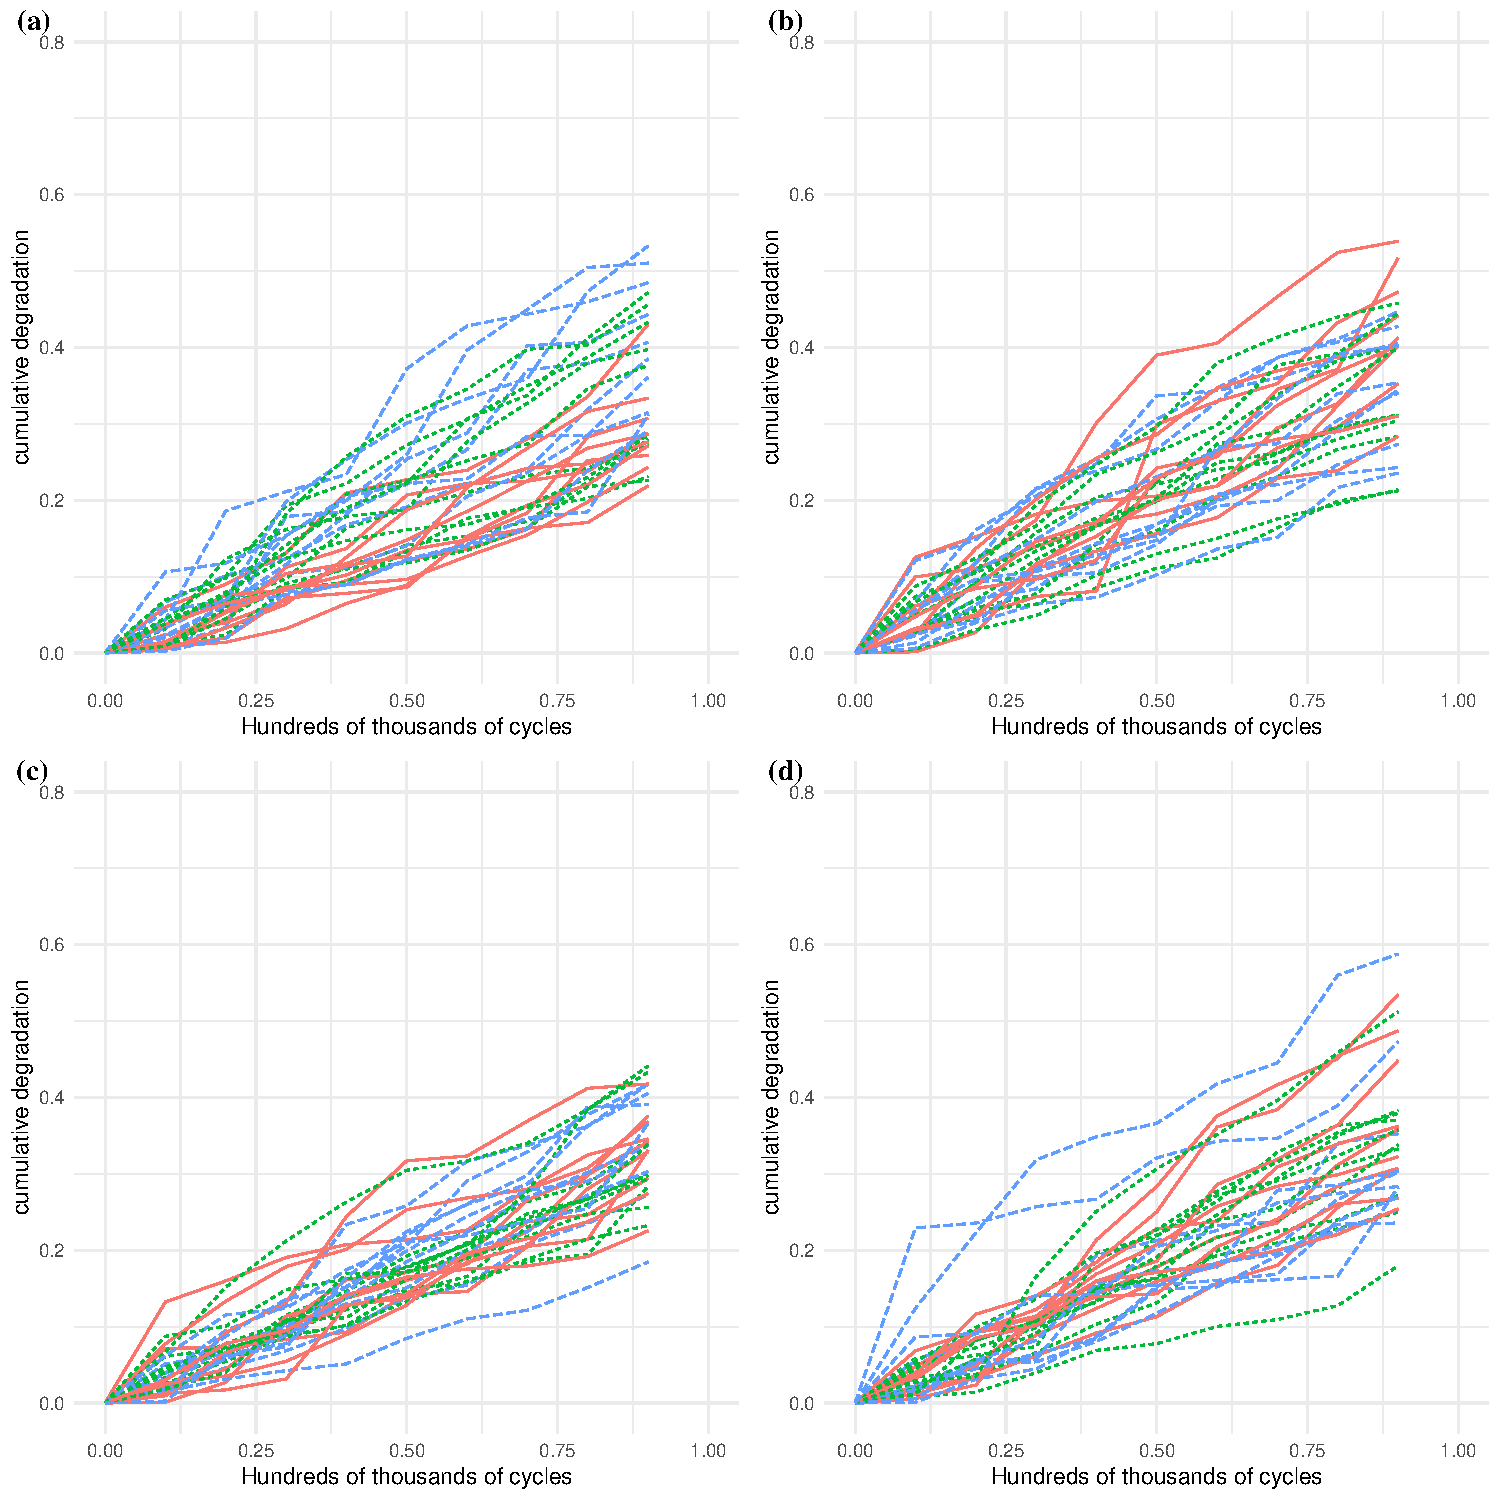
\includegraphics[width=0.95\textwidth]{./figures/ch-5/post_pc.pdf}
   \caption{Posterior predictive simulations from each of the four models. Each simulated dataset is indicated by a different colour and line type. Plot (a) shows three simulated datasets from the fitted complete pooling model, (b) from the model with varying $\mu$, (c) from the varying $\nu$ model, and (d) from the model where both $\mu$ and $\nu$ vary from unit-to-unit.}
   \label{fig:post-pc} 
\end{figure}

\subsection{Model comparison}
\label{subsec:modcomp}

Having chosen four suitable models, fitted them to the data, and checked that the sampling and inference appear reasonable, the next step is to compare the models. To do so, I use the elppd and cross-validation methods introduced in Sec.~\ref{sec:Bayesian-methods}. In the case of the crack growth data, as mentioned previously, the motivation for analysis is to predict the failure time of new units and the units currently under test but yet to fail. Doing so requires that the models predict the future degradation of the units under test and any new, unobserved units. Hence, it makes sense to compare the four models with respect to these two things.

The ability to predict the degradation of new units can be estimated from eq.~(\ref{eq:elppd_loo}) by treating the $I$ observations from each unit $j$ collectively as a single new observation, i.e., $y_j = \{y_{1j}, \ldots, y_{Ij}\}$. I refer to this method as leave-one-unit-out cross-validation ($\hbox{LOUO-CV}$) and the elppd score calculated in this way the $\hbox{elppd}_{\hbox{\tiny{LOUO-CV}}}$. By contrast, the elppd for new observations from the units under test can be approximated using eq.~(\ref{eq:elppd_loo}) by sequentially withholding the final observation, $y_{Ij}$, from each of the $J$ units; I refer to this method as step-ahead cross-validation ($\hbox{SA-CV}$) and the corresponding score as $\hbox{elppd}_{\hbox{\tiny{SA-CV}}}$. In both cases, I construct the likelihood of the withheld observations in the same way since in the data model it is assumed that the noisy observations $y_{ij}$ from the different units are independent and normally distributed conditional on the true underlying degradation, $\tilde{z}_{i, j}$, and the measurement error, $\sigma$. Although, the definition of the posterior predictive distribution of $\tilde{z}$ that should be used depends on both the cross-validation method ($\hbox{LOUO-CV}$ or $\hbox{SA-CV}$) and the model structure (i.e., complete pooling or partial pooling). The details of constructing the posterior predictive distribution of $\tilde{z}$ for $\hbox{LOUO-CV}$ or $\hbox{SA-CV}$ and the results are outlined below, and the code may be found on the GitHub repository.

\begin{table}
\centering
\caption{\label{tab:elppd_loo}Leave-one-out cross-validation statistics for the models fitted in Section~\ref{sec:unit-to-unit-sampling}.}
\centering
\begin{tabular}[t]{lrr}
\toprule
  & $\hbox{elppd}_{\hbox{\tiny{LOUO-CV}}}$ & $\hbox{elppd}_{\hbox{\tiny{SA-CV}}}$\\
\midrule
\cellcolor{gray!10}{complete pooling} & \cellcolor{gray!10}{154.3189} & \cellcolor{gray!10}{15.17704}\\
varying $\mu$ & 153.5409 & 14.00906\\
\cellcolor{gray!10}{varying $\nu$} & \cellcolor{gray!10}{153.2858} & \cellcolor{gray!10}{15.12410}\\
varying $\mu$ and $\nu$ & 153.4567 & 15.07771\\
\bottomrule
\end{tabular}
\end{table}


\paragraph{Leave-one-unit-out cross-validation} 

To calculate $\hbox{elppd}_{\hbox{\tiny{LOUO-CV}}}$, I iteratively withhold the data from each unit $j$, condition on the data from the remaining $J-1$ units and then calculate the log-likelihood of the withheld unit's observations, $y_{j} = \{y_{1j}, \ldots, y_{Ij}\}$. This calculation is based on posterior predictive draws of a new unit's (the withheld unit) filtered degradation path under the fitted model, $\tilde{z}_{j} = \{\tilde{z}_{1j}, \ldots, \tilde{z}_{Ij}\}$, and the posterior draws of $\sigma$. Thus, $\hbox{elppd}_{\hbox{\tiny{LOUO-CV}}}$ is expressed as
\begin{equation} \label{eq:elppd_louo}
 \hbox{elppd}_{\hbox{\tiny{LOUO-CV}}} = \sum^J_{j = 1}\sum^{I}_{i = 1} \log \frac{1}{S} \sum^S_{s = 1} p(y_{ij} | \left[\Tilde{z}_{ij}, \sigma \right]_{-j}^s).
\end{equation}
To generate posterior predictive draws of the non-noisy degradation path of a new unit, I sample $I-1$ jumps $\Delta\tilde{z}^s_{ij}$ in degradation from $\hbox{Ga}(\left[\tilde{\mu}_j, \tilde{\nu}_j\right]_{-i}^s)$ and then calculate their cumulative sum to generate the degradation path. If $\mu$ is completely pooled, the $\tilde{\mu}^s_j$ are taken from posterior draws $\mu^s$; similarly, if $\nu$ is completely pooled, the $\tilde{\nu}^s_j$ are posteriors draws $\nu^s$. If, however, the mean degradation varies across units, $\tilde{\mu}^s_j$ is sampled from the (hierarchical prior) $\hbox{N}^{+}(\mu^s_\mu, \sigma^s_\mu)$; in the same way, $\tilde{\nu}^s_j$ would be also sampled from $\hbox{N}^{+}(\mu_\nu, \sigma_\nu)$ if the coefficient of variation varied across units. For the models discussed in Sec.~\ref{subsec:complete-pooling} and~\ref{subsec:partial-pooling}, the first column of Tab.~\ref{tab:elppd_loo} shows the $\hbox{elppd}_{\hbox{\tiny{LOUO-CV}}}$ scores calculated in this way.

\paragraph{Step-ahead cross-validation}

Step-ahead cross-validation is carried out by iteratively withholding the most recent observation from each of the units under test, and the $\hbox{SA-CV}$ estimate of $\hbox{elppd}$ is calculated as
\begin{equation} \label{eq:elppd_sa_cv}
 \hbox{elppd}_{\hbox{\tiny{SA-CV}}} = \sum^{J}_{j = 1} \log \frac{1}{S} \sum^S_{s = 1} p(y_{Ij} | \left[\tilde{z}_{Ij}, \sigma \right]_{-\left[ Ij \right]}^s).
\end{equation}
To generate the posterior predictive draws in this case, I sample the jump in degradation for unit $j$ from $\hbox{Ga}(\mu_j, \nu_j)$ and then add this jump to the posterior draws of $\tilde{z}_{I-1,j}$. Where either $\mu$ or $\nu$ are completely pooled, $\mu_j$ and $\nu_j$ are posterior draws $\mu^s$ and $\nu^s$, respectively; otherwise, the draws from the posterior distributions of the unit-specific parameters of the gamma process are used. The $\hbox{elppd}_{\hbox{\tiny{SA-CV}}}$ scores for each of the different models are shown in the right-hand column of Table~\ref{tab:elppd_loo}.

As the $\hbox{elppd}$ results in Table~\ref{tab:elppd_loo} show, for the LOUO case, the models where $\mu$ is allowed to vary between units perform slightly better, whereas, for the SA scores, the units where $\mu$ is constant across units perform slightly better. However, the difference in both cases is marginal. The fact that the complete pooling model has the highest $\hbox{elppd}_{\hbox{\tiny{SA-CV}}}$ score---and that the inference from the complete pooling model and the partial pooling models is so similar---suggests that the completely pooled gamma process with measurement error is sufficient to model the variability in the degradation traces. However, the added variability of the unit-specific $\mu_j$ helps slightly when generalising to new units, although it is worth noting that the closeness of the models means that the $\hbox{elppd}$ results are sensitive to the priors. In \citet{leadbetter2024} we used a slightly miss-specified prior for $\mu$ and got a different result: the complete pooling model had the highest $\hbox{elppd}$ scores for both $\hbox{LOUO-CV}$ and $\hbox{SA-CV}$.

In this section, I have shown how to fit different noisy gamma process models for multiple units and demonstrated a principled way of evaluating and comparing them to identify the most appropriate one for the data set being analysed. In the case of the crack growth data, there is a marginal difference between all of the models I explore; this may not be the case for other datasets. The $\hbox{elppd}$ scores suggest that both the completely pooled and a model where $\mu$ varies between units are useful for predicting the degradation of the current units under test and new units, respectively. From both posterior predictive checking and $\hbox{elppd}$ scores, there is little motivation to allow $\nu$ to vary between units compared to the simpler constant $\nu$ alternative. Holding $\nu$ constant also results in better-behaved sampling. Therefore, in the next section, I construct failure time distributions for the units under test as well as for new units using only the complete pooling and varying $\mu$ model.

\section{Failure time distributions} \label{sec:unit-to-unit-ft}

As noted in the introduction, the crack growth measurements are collected to estimate the failure time distribution of individual units that are in-service but have not failed and/or of new units with the same nominal specifications as the experimental units. The soft failure of the terminals is considered to be when the crack length exceeds $z_f = 0.4$mm. For degradation models and a soft definition of failure, the failure time $T$ can be defined as the first passage time when the true degradation path crosses the failure threshold $z_f$\citep{balakrishnan_2017}, that is,
$$
T = \inf\left[ t|Z_t \geq z_f \right].
$$
Note that it depends on the true degradation path, not on the observed one, and hence, it does not involve the measurement error \citep{hamada_2008}. In the Bayesian context, we write the failure time distribution as $F_{T|y}(t)$, where $y = \{\{y_{ij}\}^I_{i = 1}\}^J_{j = 1}$ denotes the observed data to show that the failure time distribution is derived from the posterior distribution of the parameters and hyperparameters. It can, therefore, be written as
$$
F_{T|y}(t) = p(T < t | y) = p(Z_t > z_f | y).
$$
One of the advantages of using a fully Bayesian treatment is that we can use the posterior predictive distribution of the underlying degradation $Z_t$ to calculate the failure time distribution, thereby incorporating uncertainty in the parameters, which will be reflected in credible intervals for $F_{T|\Theta}(t)$. Alternatives to a fully Bayesian treatment include, for example, bootstrapping \citep{peng_2018}.

Although there is no explicit expression for $F_{T|y}(t)$ it is straightforward to obtain the posterior distribution of $F_{T|y}(t)$ by simulation and numerical evaluation of the distribution function of a gamma distribution (e.g., by using the R function \texttt{pgamma}), using a modified version of the procedure outlined by \citet[Sec.~8.2.1]{hamada_2008}. For the complete pooling and varying $\mu$ models, the algorithms are shown in Tab.~\ref{fig:FT_algs}.

\begin{table}
\centering
\begin{multicols}{2}

\textbf{Complete pooling}
\begin{enumerate}
    \item Draw a sample from the posterior distribution of $(\mu, \nu)$;
    \item Given that $Z_t|\mu, \nu \sim \mbox{Ga}(t/\nu^2, 1/\mu \nu^2)$, calculate $p(Z_t > z_f)$ numerically for a range of values of $t$ to generate one draw of $F_{T|y}(t)$;
    \item Repeat Steps~1. and 2. $n_{\hbox{\small{sim}}}$ times.
\end{enumerate}

\columnbreak

\textbf{Varying $\mu$}
\begin{enumerate}
    \item Draw a sample from the posterior distribution of $(\mu_\mu, \sigma_\mu, \nu)$;
    \item Generate $\mu_j$ from $\hbox{N}^{+}(\mu_\mu, \sigma_\mu)$;
    \item Using the $\mu_j$ from Step~2. and the corresponding value of $\nu$ in Step~1., generate a draw of $F_{T|y}(t)$ for a range of values of $t$ as in Step~2. for complete pooling;
    \item Repeat Steps 1.--3. $n_{\hbox{\small{sim}}}$ times.
\end{enumerate}

\end{multicols}
\caption{Algorithms for calculating the posterior distribution of the failure time distribution $F_{T|y}(t)$ for the complete pooling and varying $\mu$ models.}\label{fig:FT_algs}
\end{table}

Figure~\ref{fig:FT_CP_VM_new} shows the posterior of the failure time distributions for new units, calculated from the complete pooling and varying $\mu$ models. There is considerably greater uncertainty in $F_{T|y}(t)$ from the partial pooling model, but this is not surprising: in addition to the inherent variability of the gamma process, the partial pooling model also includes the variability in the $\mu_j$. 

\begin{figure}[h]
    \centering
    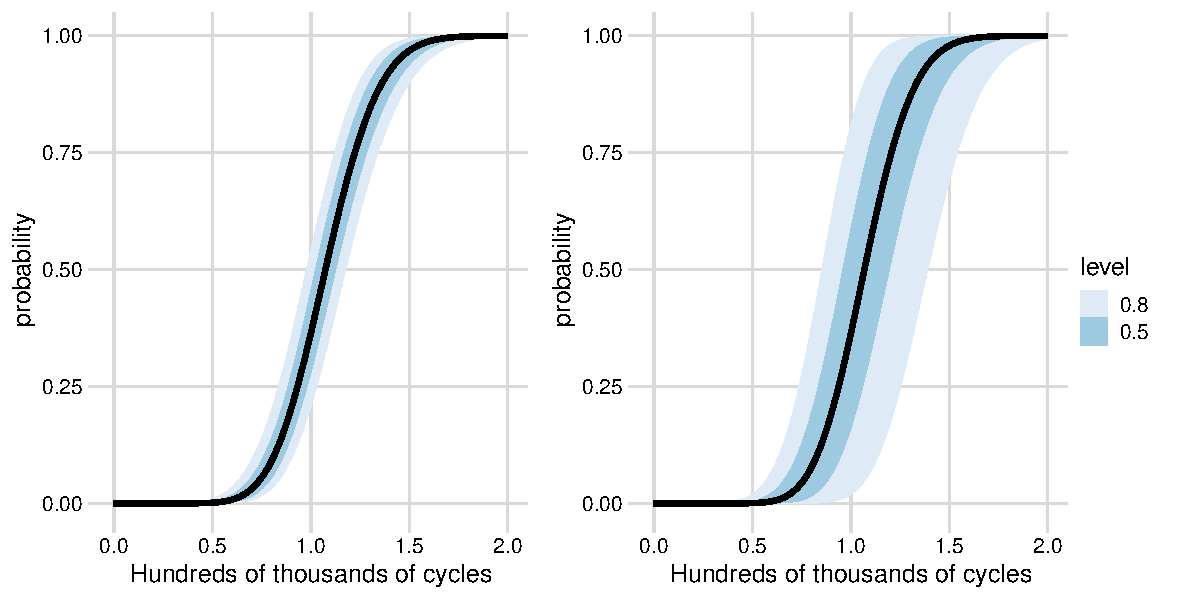
\includegraphics[width=0.95\columnwidth]{./figures/ch-5/FT_dist.pdf}
    \caption{Posterior distributions of the failure time distributions from the complete pooling model (left) and the varying $\mu$ model (right).}
    \label{fig:FT_CP_VM_new}
\end{figure}

Using slight modifications of the algorithms shown in Tab.~\ref{fig:FT_algs}, we can also calculate the failure time distribution for a unit that is currently under test and that has yet to fail, for example, Unit 3. This distribution, also known as the predictive failure time distribution\citep{lawless2004}, is conditional on the unit not having failed by $t_I$ and having attained a degradation level $z_I$. Since $z_I$ is a latent variable in the model, the posterior distribution contains samples of $z_I$ from which we can calculate the jump in degradation that corresponds to a soft failure. Figure~\ref{fig:FT_CP_VM_U3} shows the posterior predictive failure time distributions for Unit 3, which has not failed; again, we see that because of the additional layer of uncertainty, the credible intervals for the varying $\mu$ model are wider than those from the complete pooling model, although the difference is not as extreme compared to the failure time distributions for new units. Comparing Fig.~\ref{fig:FT_CP_VM_new} with Fig.~\ref{fig:FT_CP_VM_U3}, the unit-specific failure time distributions have tighter uncertainty intervals than their new unit counterparts. This difference is more significant for the varying $\mu$ model since the unit-specific estimate does not average over the variability in the $\mu_j$ and so is a much more precise estimate.

\begin{figure}[h]
    \centering
    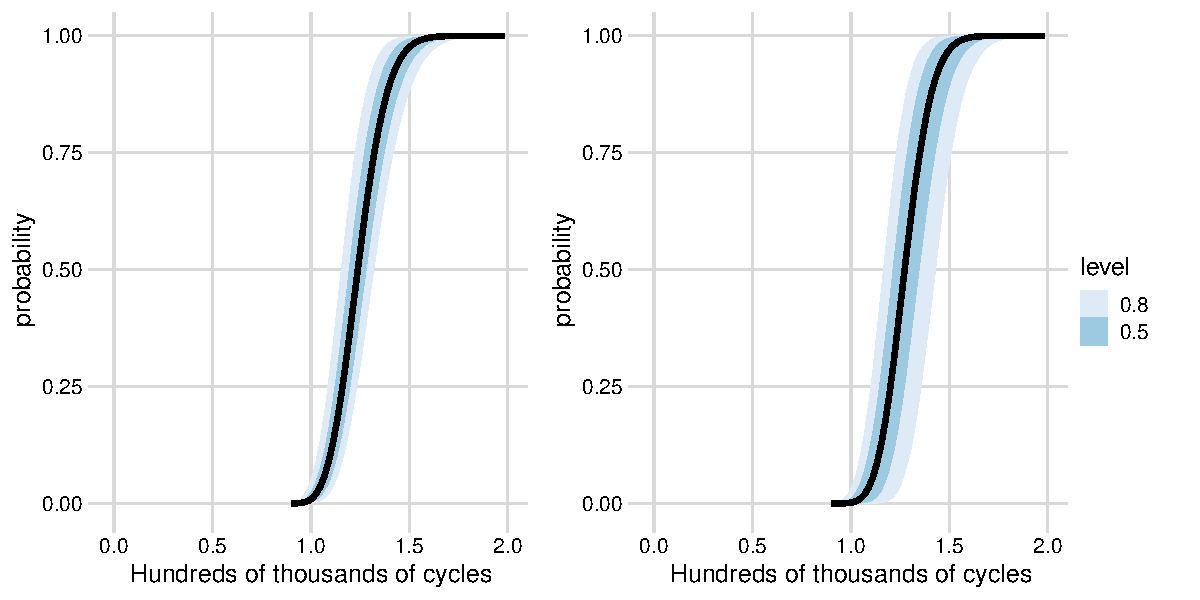
\includegraphics[width=0.95\columnwidth]{./figures/ch-5/FT_dist_Unit3.pdf}
    \caption{Posterior distributions of the predictive failure time distributions from the complete pooling model (left) and the varying $\mu$ model (right) for Unit~3.}
    \label{fig:FT_CP_VM_U3}
\end{figure}

\section{Discussions} \label{sec:unit-to-unit-discussion}

In this chapter, I showed how the noisy gamma process model for a single degradation path from Chap.~\ref{chap:chapter4} could be extended---using the same hierarchical modelling framework---to incorporate unit-to-unit variability when modelling the noisy degradation traces of multiple nominally-identical units, and how allowing some parameters to vary determines how information is shared between observational units. I then demonstrated the fitting, evaluation, and comparison of these models on an experimental crack growth dataset with added measurement error. Lastly, I showed how failure time distributions (with uncertainty bands) can be constructed for both new units and units under test using the posterior distributions of either a complete pooling or partial pooling gamma process model. This final section reviews the chapter's main points and discusses the key findings, contributions, and areas for future work.

To model the ten units' noisy degradation traces in Fig.~\ref{fig:crack-growth-w-noise} simultaneously, I explored several models: one where all of the degradation traces arise from the same underlying gamma process (complete pooling) and others where either $\mu$, $\nu$, or both are allowed to vary between units (partial pooling). Parameterising the gamma process in terms of $\mu$ and $\nu$ clarifies how unit-to-unit variability can be incorporated into the model and forces the analyst to be explicit in how he/she expect the units to vary: should the mean wear rate vary among units, or the volatility? In the same way, the new parameterisation also clarifies how we might model the effect of covariates on the degradation: for example, should environmental variables such as varying temperature or humidity affect the mean wear or the volatility? There are no covariates for the crack growth data, but extending the BHM to include covariate information would be interesting future work if data were available to do so. The fact that parameters $\mu$ and $\nu$ have clear and separate effects also helped diagnose the sampling issues and interpret the posterior of the parameters and hyperparameters directly.

Based on the elppd criterion, the models where $\mu$ varies between units perform best for predicting out-of-sample. In contrast, models where $\mu$ is constant across observational units best predict the future observations of the units under test. Although, the differences in the elppd scores are relatively small. All of the models explored fit the data: the predictive distributions of each unit's underlying degradation path contains the true degradation path, and the marginal posterior of $\sigma$ include the true value $\sigma = 0.025$. In the posterior distributions of the partial pooling models, there is evidence that $\mu$ should be allowed to vary between units since there is some variability in the modes of the marginal posteriors of the unit-specific $\mu_j$. However, the spread of these distributions are wide enough to encompass the mean $\mu_\mu$---in addition, the posterior of $\sigma_\mu$ has mass near zero---therefore it could well be that all units share the same $\mu_i$ value, even under a model where we allow them to vary. In the models where $\nu$ varies, the marginal posterior distributions of the unit specific $\nu_j$ are almost identical, and the marginal posterior of $\sigma_\nu$ has considerable mass near zero, showing that there is little evidence that the coefficient of variation varies among the units.

Given the weak evidence in the hierarchical models' posteriors that $\mu$ varies from unit-to-unit, and even weaker evidence that $\nu$ varies, it is understandable that the complete pooling model performs at the same level as the partial pooling models for the crack growth data. The complete pooling model performs best in the case of $\hbox{elppd}_\text{SA-CV}$, possibly because assuming the simpler model structure results in the data more strongly informing the three parameters and hence more precisely estimating the volatility of the gamma process ($\nu$): which is important for accurately forecasting future degradation. Because of the marginal difference between the four models, it is not surprising that in \citet{leadbetter2024}, where we used a slightly different prior for $\mu$, the complete pooling model performs best with respect to both $\hbox{elppd}_\text{LOUO-CV}$ and $\hbox{elppd}_\text{SA-CV}$; showing that the ordering is sensitive to the model specification and prior. \citet{rodriguez-picon2018} analyses the same data using gamma processes that incorporate unit-to-unit variability but without measurement error. They find that, when the data do not include measurement error, one of the partial-pooling models they explore outperforms the complete pooling model according to information criteria methods. However, there is also very little difference among the models they explore.

The struggle to clearly identify the best model could be a result of the nested structure of the models. When the observed variability of the degradation traces can easily be explained by the complete pooling model (which appears to be the case for the crack growth data), all of the models I have explored here contain this `true' model. Future work exploring how well the elppd methods identify the true model from complete and partial pooling models when the data are generated from one or the other would be interesting. The presence of measurement error adds an additional \emph{degree of freedom} to the models, making it even more difficult to clearly identify the best \emph{underlying} model candidate. To this end, it would also be helpful if future work exploring elppd through simulation looked at the effect of sample size and noise level on how clearly the true model is identified. In an early work on unit-to-unit variability, \citet{lawless2004} devise a statistical test to determine whether or not a random effect should be included in a degradation model when working in a non-Bayesian framework. Similar guidance for Bayesian models could be helpful.

The crack growth data that I have analysed do not show strong signs that there is variability among the units outside of the usual `jumpiness' of a gamma process. For other data, identifying a suitable partial pooling model may be much more obvious. Nevertheless, I have shown how analysts can propose, fit, check, and then, finally, choose between suitable Bayesian model candidates using a fully Bayesian framework.
